\documentclass[a4paper,12pt,oneside]{book}
\usepackage[italian]{babel}
\usepackage[utf8]{inputenc}
\usepackage{textcomp}
\usepackage[parfill]{parskip} %Se necessatrio non indenta, ma inserisce spazio
\usepackage{graphicx}
\usepackage{hyperref}
\usepackage{amsmath} %To number equations

\usepackage{titling}
\newcommand{\subtitle}[1]{%
 \posttitle{%
 \par\end{center}
 \begin{center}\large#1\end{center}
 \vskip6.5em}%
}

\author{Andrea Onofri}
\date{2018-12-10}
\title{Metodologia di sperimentazione in agricoltura}
\subtitle{}


%***************************************************************

%Specific RMarkdown
\usepackage{color}
\usepackage{fancyvrb}
\usepackage{longtable}
\usepackage{booktabs}
\providecommand{\tightlist}{%
  \setlength{\itemsep}{0pt}\setlength{\parskip}{0pt}}
\newcommand{\VerbBar}{|}
\newcommand{\VERB}{\Verb[commandchars=\\\{\}]}
\DefineVerbatimEnvironment{Highlighting}{Verbatim}{commandchars=\\\{\}}
\usepackage{framed}
\definecolor{shadecolor}{RGB}{248,248,248}
\newenvironment{Shaded}{\begin{snugshade}}{\end{snugshade}}
\newcommand{\KeywordTok}[1]{\textcolor[rgb]{0.13,0.29,0.53}{\textbf{#1}}}
\newcommand{\DataTypeTok}[1]{\textcolor[rgb]{0.13,0.29,0.53}{#1}}
\newcommand{\DecValTok}[1]{\textcolor[rgb]{0.00,0.00,0.81}{#1}}
\newcommand{\BaseNTok}[1]{\textcolor[rgb]{0.00,0.00,0.81}{#1}}
\newcommand{\FloatTok}[1]{\textcolor[rgb]{0.00,0.00,0.81}{#1}}
\newcommand{\ConstantTok}[1]{\textcolor[rgb]{0.00,0.00,0.00}{#1}}
\newcommand{\CharTok}[1]{\textcolor[rgb]{0.31,0.60,0.02}{#1}}
\newcommand{\SpecialCharTok}[1]{\textcolor[rgb]{0.00,0.00,0.00}{#1}}
\newcommand{\StringTok}[1]{\textcolor[rgb]{0.31,0.60,0.02}{#1}}
\newcommand{\VerbatimStringTok}[1]{\textcolor[rgb]{0.31,0.60,0.02}{#1}}
\newcommand{\SpecialStringTok}[1]{\textcolor[rgb]{0.31,0.60,0.02}{#1}}
\newcommand{\ImportTok}[1]{#1}
\newcommand{\CommentTok}[1]{\textcolor[rgb]{0.56,0.35,0.01}{\textit{#1}}}
\newcommand{\DocumentationTok}[1]{\textcolor[rgb]{0.56,0.35,0.01}{\textbf{\textit{#1}}}}
\newcommand{\AnnotationTok}[1]{\textcolor[rgb]{0.56,0.35,0.01}{\textbf{\textit{#1}}}}
\newcommand{\CommentVarTok}[1]{\textcolor[rgb]{0.56,0.35,0.01}{\textbf{\textit{#1}}}}
\newcommand{\OtherTok}[1]{\textcolor[rgb]{0.56,0.35,0.01}{#1}}
\newcommand{\FunctionTok}[1]{\textcolor[rgb]{0.00,0.00,0.00}{#1}}
\newcommand{\VariableTok}[1]{\textcolor[rgb]{0.00,0.00,0.00}{#1}}
\newcommand{\ControlFlowTok}[1]{\textcolor[rgb]{0.13,0.29,0.53}{\textbf{#1}}}
\newcommand{\OperatorTok}[1]{\textcolor[rgb]{0.81,0.36,0.00}{\textbf{#1}}}
\newcommand{\BuiltInTok}[1]{#1}
\newcommand{\ExtensionTok}[1]{#1}
\newcommand{\PreprocessorTok}[1]{\textcolor[rgb]{0.56,0.35,0.01}{\textit{#1}}}
\newcommand{\AttributeTok}[1]{\textcolor[rgb]{0.77,0.63,0.00}{#1}}
\newcommand{\RegionMarkerTok}[1]{#1}
\newcommand{\InformationTok}[1]{\textcolor[rgb]{0.56,0.35,0.01}{\textbf{\textit{#1}}}}
\newcommand{\WarningTok}[1]{\textcolor[rgb]{0.56,0.35,0.01}{\textbf{\textit{#1}}}}
\newcommand{\AlertTok}[1]{\textcolor[rgb]{0.94,0.16,0.16}{#1}}
\newcommand{\ErrorTok}[1]{\textcolor[rgb]{0.64,0.00,0.00}{\textbf{#1}}}
\newcommand{\NormalTok}[1]{#1}
% Redefine \includegraphics so that, unless explicit options are
% given, the image width will not exceed the width of the page.
% Images get their normal width if they fit onto the page, but
% are scaled down if they would overflow the margins.


\begin{document}

\maketitle
\tableofcontents

\chapter{Introduzione}\label{introduzione}

\section{Organizzazione del corso}\label{organizzazione-del-corso}

Questo corso si compone di due parti, che sono trattate in parziale
sovrapposizione durante durante il semestre. Nella prima parte, sono
fornite le basi teoriche e gli strumenti pratici per pianificare,
organizzare e condurre esperimenti scientifici nel settore agrario.

Nella seconda parte, dopo un'introduzione agli argomenti generali
relativi alla biostatistica, ci occupiamo dell'analisi e
dell'interpretazione dei dati ottenuti nelle prove scientifiche, nonché
della presentazione dei risultati tramite tesi, report e/o pubblicazione
scientifica. In questa seconda parte, daremo ampio spazio all'impiego di
modelli matematici interpretativi, utilizzati sia con finalità
descrittive, sia con finalità predittive.

\section{Esercitazioni pratiche}\label{esercitazioni-pratiche}

Questo corso non ha finalità puramente teoriche, ma fondamentalmente
pratiche, improntate al `saper fare'. In sostanza, all fine del corso,
gli studenti dovranno essere in grado di pianificare esperimenti ed
analizzarne i risultati. E'importante quindi lavorare con alcuni casi
studio relativi ad esperimenti molto comuni in ambito agrario, come le
prove varietali, le prove di concimazione, le prove di diserbo, i
dosaggi biologici e i saggi germinativi.

Per poter risolvere gli esempi proposti, lo studente dovrà quindi
avvalersi di un opportuno software statistiche. In questo caso, abbiamo
due proposte: Excel (molto comune) e R (freeware e molto avanzato). A
lezione tratteremo prevalentemente R, ma gli studenti, soprattutto
quelli che non seguono le lezioni, potranno anche affidarsi ad Excel. In
questa dispensa proporremo soluzioni per entrambi i software.

\section*{Obiettivi specifici del
Corso}\label{obiettivi-specifici-del-corso}
\addcontentsline{toc}{section}{Obiettivi specifici del Corso}

Come dicevamo, il Corso ha un contenuto prettamente tecnico e gli
obiettivi specifici sono fondamentalmente pratici, con una forte
attenzione al `saper fare'.

Gli studenti dovranno:

\begin{enumerate}
\def\labelenumi{\arabic{enumi}.}
\tightlist
\item
  Rispondere a domande generali sulla metodologia sperimentale e
  sull'organizzazione degli esperimenti
\item
  Saper disegnare correttamente l'esperimento proposto (uno), scegliendo
  adeguatamente il layout sperimentale (disegno, numero di repliche) e
  disegnando la mappa in modo corretto. Gli esperimenti proposto
  apparterranno alle seguenti categorie: prove di confronto varietale,
  prove di confronto tra erbicidi, prove di degradazione dei
  fitofarmaci, dosaggi biologici con erbicidi, prove di concimazione,
  prove di epoca di semina;
\item
  Saper eseguire l'ANOVA per il dataset proposto (uno), scelto tra
  quelli riportati nell'apposito elenco;
\item
  Saper adattare il modello opportuno (lineare o nonlineare) ad un
  dataset assegnato, scelto tra quelli riportati nell'apposito elenco.
  Saper valutare la bontà di adattamento del modello.
\end{enumerate}

Per il punto 3 e il punto 4 gli studenti si dovranno avvalere di un
supporto informatico, ad esempio costituito dal software R (citation) o
da Excel, con la macro DSAASTAT (per l'ANOVA).

\chapter{Il metodo sperimentale: quando la scienza è
scienza}\label{il-metodo-sperimentale-quando-la-scienza-e-scienza}

\section{Introduzione}\label{introduzione-1}

In una società caratterizzata dal sovraccarico cognitivo immagino sia
giusto chiedersi (e chiedere) che cosa sia la scienza, cosa distingua le
informazioni scientifiche da tutto quello che invece non è altro che
pura opinione, magari autorevole, ma senza il sigillo dell'oggettività.

Per quanto affascinante possa sembrare l'idea del ricercatore che con
un'improvviso colpo di genio elabora una stupefacente teoria, dovrebbe
essere chiaro che l'intuizione è solo un possibile punto di partenza,
che non necessariamente prelude al progresso scientifico, per quanto
geniale ed innovativa possa essere. In generale, almeno in ambito
biologico, nessuna teoria acquisisce automaticamente valenza
scientifica, ma rimane solo nell'ambito delle opinioni,
indipendentemente dal fatto che nasca da un colpo di genio, oppure
grazie ad un paziente e meticoloso lavoro di analisi intellettuale, che
magari si concretizza in un modello matematico altamente elegante e
complesso.

Da un punto di vista puramente intuitivo, è ovvio aspettarsi che una
prova scientifica debba uscire dall'ambito delle opinioni legate a
divergenze di cultura, percezione e/o credenze individuali, per
divenire, al contrario, oggettiva e universalmente valida,
distinguendosi quindi da altre verità di natura metafisica, religiosa o
pseudoscientifica. Che cosa è che permette alla scienza di divenire
tale?

A questo proposito, riporto alcuni aforismi significativi:

\begin{enumerate}
\def\labelenumi{\arabic{enumi}.}
\tightlist
\item
  Proof is a justified true belief (Platone, Dialoghi)
\item
  The interest I have in believing a thing is not a proof of the
  existence of that thing (Voltaire)
\item
  A witty saying proves nothing (Voltaire)
\end{enumerate}

\subsection{Cosa è quindi una prova
scientifica?}\label{cosa-e-quindi-una-prova-scientifica}

La base di tutta la scienza risiede nel cosiddetto `metodo scientifico',
che si fa comunemente risalire a Galileo Galilei (1564-1642) e che è
riassunto nella figura seguente.

\begin{figure}
\centering
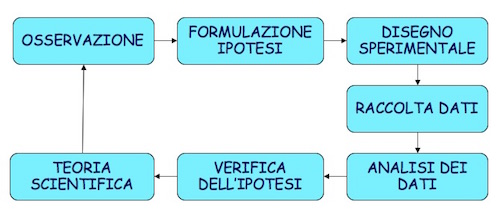
\includegraphics[width=0.75000\textwidth]{_images/MSAMap.jpg}
\caption{Il metodo scientifico Galileiano}
\end{figure}

Senza andare troppo in profondità, è importante notare due aspetti:

\begin{enumerate}
\def\labelenumi{\arabic{enumi}.}
\tightlist
\item
  il ruolo fondamentale dell'esperimento scientifico, che produce dati a
  supporto di ipotesi pre-esistenti;
\item
  lo sviluppo di teorie basate sui dati, che rimangono valide fino a che
  non si raccolgono altri dati che le confutano, facendo nascere nuove
  ipotesi che possono portare allo sviluppo di nuove teorie, più
  affidabili o più semplici.
\end{enumerate}

Insomma, l'ingrediente fondamentale di una prova scientifica è che è
supportata da un insieme dei dati sperimentali; di fatto, non esiste
scienza senza dati! Resta famoso l'aforisma ``In God we trust, all the
others bring data'', attribuito all'ingegnere e statistico americano W.
Edwards Deming (1999-1923), anche se pare che egli in realtà non l'abbia
mai pronunciato.

\section{Esperimenti buoni e
cattivi!}\label{esperimenti-buoni-e-cattivi}

Non tutti gli esperimenti sono buoni e, di conseguenza, non tutti i dati
sono buoni. In particolare, due sono gli elementi che possono portare a
dati di diversa affidabilità:

\begin{enumerate}
\def\labelenumi{\arabic{enumi}.}
\tightlist
\item
  Errore sperimentale
\item
  Campionamento
\end{enumerate}

Vediamo qualche dettaglio in più a proposito di questi due elementi.

\subsection{L'errore sperimentale}\label{lerrore-sperimentale}

Alla base della raccolta di dati sperimentali vi è un processo di
\textbf{misurazione}, attraverso la quale il fenomeno oggetto di studio
viene caratterizzato con appositi strumenti scientifici, più o meno
complessi. Il problema è che nessuna misura può essere considerata
precisa in senso assoluto, cioè perfettamente coincidente col valore
reale della grandezza misurata, che è destinato a rimanere un'entità
incognita e indeterminabile.

In particolare, in ogni esperimento scientifico esiste un potenziale
elemento di confusione che gli scienziati conoscono con il termine di
\textbf{errore sperimentale}, con la cui presenza è necessario
confrontarsi sempre e comunque.

Nel misurare una determinata grandezza fisica, indipendentemente dal
metodo scelto per la misura, possiamo sempre commettere due tipi di
errore: \textbf{sistematico} ed \textbf{accidentale (casuale)}.

L'errore sistematico è provocato da difetti intrinseci dello strumento o
incapacità peculiari dell'operatore e tende a ripetersi costantemente in
misure successive. Un esempio tipico è quello di una bilancia non
tarata, che tende ad aggiungere 20 grammi ad ogni misura che
effettuiamo. Per queste sue peculiarità, l'errore sistematico non è
quantificabile e deve essere contenuto al minimo livello possibile
tramite la perfetta taratura degli strumenti e l'adozione di metodi di
misura rigidamente standardizzati e accettati dalla comunità scientifica
mondiale.

L'errore accidentale (o casuale) è invece legato a fattori variabili nel
tempo e nello spazio, quali:

\begin{enumerate}
\def\labelenumi{\arabic{enumi}.}
\tightlist
\item
  \emph{malfunzionamenti accidentali dello strumento}. Si pensi ad
  esempio al rumore elettrico di uno strumento, che fa fluttuare i
  risultati delle misure effettuate;
\item
  \emph{imprecisioni o disattenzioni casuali dell'operatore}. Si pensi
  ad esempio ad un banale errore di lettura dello strumento, che può
  capitare soprattutto ad un operatore che esegua moltissime misure
  manuali con procedure di routine;
\item
  \emph{irregolarità} dell'oggetto da misurare\} unite ad una precisione
  relativamente elevata dello strumento di misura. Si pensi alla
  misurazione del diametro di un melone con un calibro: è facile che
  compaiano errori legati all'irregolarità del frutto o al fatto che
  l'operatore non riesce a misurare lo stesso nel punto in cui il suo
  diametro è massimo. Oppure, più semplicemente si pensi alla
  misurazione della produzione di granella di una certa varietà di
  frumento: anche ipotizzando di avere uno strumenti di misura perfetto
  e quindi esente da errore, la produzione mostrerebbe comunque una
  fluttuazione naturale da pianta a pianta, in base al patrimonio
  genetico e, soprattutto, in base alle condizioni di coltivazione che
  non possono essere standardizzate oltre ad un certo livello (si pensi
  alla variabilità del terreno agrario).
\end{enumerate}

Dato che queste imprecisioni sono assolutamente casuali è chiaro che le
fluttuazioni positive (misura maggiore di quella vera) sono altrettanto
probabili di quelle negative e tendono a presentarsi con la stessa
frequenza quando si ripetano le misure più volte. Di conseguenza,
l'errore sperimentale casuale può essere gestito attraverso la
\textbf{replicazione delle misure}: infatti, se ripeto una misura
soggetta a questo tipo di errore, nel lungo periodo gli errori positivi
e negativi tendono ad annullarsi reciprocamente e la media delle misure
effettuate tende quindi a coincidero con il valore reale della grandezza
da misurare.

\subsection{Il campionamento}\label{il-campionamento}

Se è vero, e la pratica sperimentale lo conferma, che ripetere le misure
porta ad ottenere molti risultati diversi, nasce il problema di capire
quante repliche sono necessarie. Se si ripensa a quanto detto finora,
dovrebbe risultare evidente che, per ottenere una misura pari
all'effettivo (reale) valore della grandezza da misurare, bisognerebbe
effettuarne infinite. Tuttavia è altrettanto evidente che questo
procedimento è totalmente improponibile!!!

Qual è la strada seguita dagli scenziati, quindi? E' quella di
raccogliere un numero finito di misure, sufficientemente basso da essere
compatibile con le umane risorse di tempo e denaro, ma sufficientemente
alto da essere giudicato attendibile. Qualunque sia questo valore
finito, è evidente che ci troviamo difronte solo ad un campione delle
infinite misure che avremmo dovuto fare, ma che non abbiamo fatto. La
domanda è: questo campione è rappresentativo o no? E' in grado di
descrivere adeguatamente la realtà? E' possibile che gli errori
sperimentali positivi e negativi non si siano annullati tra loro,
confondendosi con l'effetto biologico in studio? In altre parole:
possiamo fidarci dei dati che abbiamo raccolto?

La possibilità di raccogliere dati sbagliati è tutt'altro che remota.
Gli scienziati american Pons e Fleischmann il 23 Marzo del 1989
diffusero pubblicamente la notizia di essere riusciti a riprodurre la
fusione nucleare fredda, causando elevatissimo interesse nella comunità
scientifica. Purtroppo le loro misure erano vizite da una serie di
problemi e il loro risultato fu clamorosamente smentito da esperimenti
successivi.

\begin{figure}
\centering
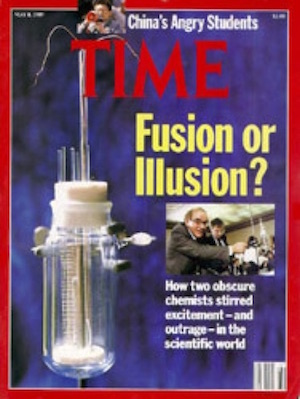
\includegraphics[width=0.50000\textwidth]{_images/FalseResults.jpg}
\caption{Conseguenze di un esperimento sbagliato}
\end{figure}

\section{Scienza = metodo}\label{scienza-metodo}

Insomma, la scienza deve essere basata sui dati, ma i dati contengono
inevitabili fonti di incertezza, legate all'errore sperimentale e al
processo di campionamento. Come si può procedere in queste condizioni?
Il punto fondamentale è quello di adottare un metodo sperimentale che
consenta di ottenere dati \textbf{il più affidabili possibile}. Insomma,
questa semplice affermazione significa che bisogna fare eseperimenti ben
condotti, precisi, seguendo procedure standardizzate e/o largamente
condivise dalla comunità scientifica.

Certo è che, per quanto detto in precedenza, il fatto che i dati
provengano da un processo di campionamento impedisce, di fatto, di
ottenere un'affidabilità totale. Cosa succederebbe se ripetessimo
l'esperimento?

Insomma, bisogna fare alcune considerazioni, che elenco di seguito:

\begin{enumerate}
\def\labelenumi{\arabic{enumi}.}
\tightlist
\item
  in primo luogo si dovrà accettare il fatto che, contrariamente a
  quanto si potrebbe o vorrebbe credere, non esistono prove scientifiche
  totalmente certe, ma l'incertezza è un elemento intrinseco della
  scienza.
\item
  In secondo luogo si dovranno utilizzare gli strumenti della statistica
  necessari per quantificare l'incertezza residua, che dovrà essere
  sempre riportata a corredo dei risultati di ogni esperimento
  scientifico.
\item
  Ogni risultato sarà quindi valutato dalla comunità scientifica sullo
  sfondo della sua incertezza, seguendo alcune regole di natura
  probabilistica che consentono di stabilire se la prova scientifica è
  sufficientemente forte per essere considerata tale.
\end{enumerate}

Un elemento fondamentale di valutazione della bontà di un esperimento e
dei dati da esso ottenuti sta nella cosiddetta \textbf{replicabilità},
cioè nella probabilità di ottenere risultati molto simili (se non
uguali) replicando l'esperimento in condizioni analoghe. Per valutare se
un esperimento è replicabile è necessario che questo sia descritto con
un grado di dettaglio tale da permettere a chinque di ripeterlo,
ottenendo risultati comparabili e non contraddittori. Nessun risultato
di cui non sia provata la riproducibilità è da considerarsi valido.

E'chiaro comunque che ogni esperimento può essere smentito. Questo non è
un problema: la scienza è pronta a considerare una prova scientifica
valida fino a che non si raccolgono dati altrettanto affidabili che la
confutino. In questo caso, si abbandona la teoria confutata e si
abbraccia la nuova. L'abbandono può anche non essere totale: ad esempio
la teoria gravitazionale di Newton è ancora oggi valida per molto
situazioni pratiche, anche se è stata abbandonoata in favore della
teoria della relatività, che spiega meglio il moto dei corpi ad
altissime velocità.

In effetti, la scienza considere sempre con attenzione il principio del
rasoio di Occam, per il quale si accetta sempre la teoria più semplice
per interpretare una dato fenomeno, riservando le teorie più complesse
alle situazioni più difficili, che giustificano tale livello di
complessità.

\section{Chi valuta se un esperimento è
attendibile?}\label{chi-valuta-se-un-esperimento-e-attendibile}

Quanto detto finora vorrebbe chiarire come il punto centrale della
scienza non è la certezza delle teorie, bensì il metodo che viene
utilizzato per definirle. Ognuno di noi è quindi responsabile di
verificare che le informazioni in suo possesso siano `scientificamente'
attendibili, cioè ottenute con un metodo sperimentale adeguato. Il fatto
è che non sempre siamo in grado di compiere questa verifica, perché non
abbiamo strumenti `culturali' adeguati, se non nel ristretto ambito
delle nostre competenze professionali. Come fare allora?

L'unica risposta accettabile è quella di controllare l'attendibilità
delle fonti di informazione. In ambito biologico, le riviste autorevoli
sono caratterizzate dal procedimento di `\emph{peer review}', nel quale
i manoscritti scientifici, prima della pubblicazione, sono sottoposti ad
un comitato editoriale ed assegnati ad un `editor', il quale legge il
lavoro e contemporaneamente lo invia a due o tre scienziati anonimi e
particolarmente competenti in quello specifico settore scientifico
(\emph{reviewers} o revisori).

I revisori, insieme all'\emph{editor}, compiono un attento lavoro di
esame e stabiliscono se l'evidenza scientifica presentata è
sufficientemente `forte'. Le eventuali critiche vengono presentate
all'autore, che è tenuto a rispondere in modo convincente, anche
ripetendo gli esperimenti se necessario. Il processo richiede spesso
interi mesi ed è abbastanza impegnativo per uno scenziato. E' piuttosto
significativa l'immagine presentata in
\href{http://scienceblogs.com/startswithabang/2013/06/07/the-4-jobs-of-a-referee-in-peer-review/}{scienceBlog.com},
che allego qui.

\begin{figure}
\centering
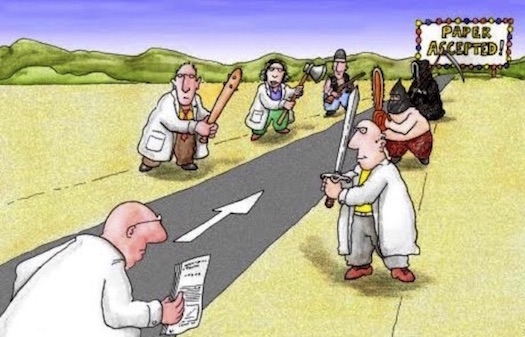
\includegraphics[width=0.75000\textwidth]{_images/PeerReview.jpg}
\caption{Il processo di \emph{peer review}}
\end{figure}

In sostanza il meccanismo di \emph{peer review} è l'analogo scientifico
di un processo, nel quale l'inputato (lavoro scientifico) viene assolto
(rilasciato, leggi: rigettato) in presenza di qualunque ragionevole
dubbio metodologico. Attenzione: il dubbio che non deve esistere è
quello metodologico, dato che il dubbio sul risultato non può essere
allontanato completamente e i reviewer controlleranno solo che esso si
trovi al disotto della soglia massima, stabilita con metodiche
statistiche.

Questo procedimento, se effettuato con competenza, dovrebbe aiutare a
separare la scienza dalla pseudo-scienza e, comunque, ad eliminare la
gran parte degli errori metodologici dai lavori scientifici.

\section{Il metodo sperimentale}\label{il-metodo-sperimentale}

Almeno in ambito biologico, la definizione del metodo sperimentale è
fondamentalmente attribuita allo scienziato inglese Ronald Fisher
(1890-1962), che l'ha esplicitata nel suo famoso testo del 1935 (The
design of experiments). Mi sembra opportuno riassumerla nelle tre
espressioni `chiave': controllo locale degli errori, replicazione e
randomizzazione. Si tratta di:

\begin{enumerate}
\def\labelenumi{\arabic{enumi}.}
\tightlist
\item
  contenere al massimo possibile l'errore sperimentale, con l'adozione
  di tecniche opportune, in modo da separare le fonti di variabilità,
  isolando qualla oggetto di studio (controllo locale degli errori);
\item
  replicare le misure più volte (replicazione)
\item
  Scegliere le unità sperimentali da misurare in modo totalmente
  casuale, così da avere un campione rappresentativo ed evitare di
  confondere gli effetti prodotti dall'errore sperimentale con quelli
  prodotti dal fenomeno biologico oggetto di studio (randomizzazione)
\end{enumerate}

Vediamo ora un'esempio banale di come procedere.

\section{Metodi sperimentali validi ed
invalidi}\label{metodi-sperimentali-validi-ed-invalidi}

Immaginiamo un ricercatore che abbia un'idea brillante: egli ha
inventato un nuovo fertilizzante `prodigioso'. E' evidente che non può
presentarsi alla comunità scientifica declamando le doti di questo
fertilizzante, in quanto egli verrebbe immediatamente esposto al
pubblico ludibrio, perchè sta presentando delle opinioni, non delle
evidenze scientifiche (almeno, così dovrebbe essere, in una società
sana\ldots{} purtroppo in un'era di pseudo-scienza siamo sempre pronti a
dar credito a chiunque, senza un'adeguata dose di scetticismo\ldots{} )

\subsection{Primo esperimento}\label{primo-esperimento}

Come ogni scenziato, egli deve raccogliere dati. E lo fa, organizzando
un esperimento, nel quale prende un campo di mais e lo fertilizza con il
suo nuovo composto, ritraendo una produzione del 20\% superiore a quella
usuale. Ovvoamente, se prova a pubblicare questa notizia, il suo lavoro
verrà certamente (si spera\ldots{}) rigettato, in quanto rimane il
dubbio su chi sia la causa dell'effetto riscontrato: il fertilizzante?
il clima dell'anno di prova? il suolo? la varietà di mais impiegata? E'
chiaro che questo non è un esperimento controllato: il campo trattato e
quello non trattato (riferimento) non sono totalmente uguale, eccetto
che per il fertilizzante impiegato.

\subsection{Secondo esperimento}\label{secondo-esperimento}

A questo punto il ricercatore pianifica un esperimento comparativo
controllato: prende due campio di mais, vicini, con lo stesso terreno,
semina la stessa varietà di mais e coltiva i due campi esattamente nello
stesso modo, con l'unica differenza che in uno di essi somministra il
fertilizzante in studio (campo trattato) e nell'altro no (testimone o
controllo). Alla fine osserva che il campo trattato produce 130
tonnellate per ettaro, mentre quello non trattato ne produce 115 e
conclude che il nuovo fertilizzante è efficace (+ 12\% circa). Infatti
egli ritiene che, dato che i due campi sono totalmente uguali,
l'incremento di produzione non possa che essere attribuito al
fertilizzante. Scrive un report, che, purtroppo, viene rigettato.

Anche se questo secondo esperimento è meglio del primo, permane tuttavia
il dubbio che l'effetto si sia prodotto per caso. Potrebbe infatti
esserci stata una qualche situazione non osservata che ha avvantaggiato
uno dei due campi. Ad esempio un attacco di insetti, una carenza idrica,
o qualsivoglia altra situazione. Questo vi sembra improbabile? Non
importa, con una sola osservazione il ricercatore non è in grado di
provare che il risultato è replicabile.

\subsection{Terzo esperimento}\label{terzo-esperimento}

Avendo imparato la lezione, il ricercatore fa un nuovo esperimento,
utilizzando stavolta otto campi: quattro trattati e quattro non
trattati. Anche in questo caso osserva un incremento produttivo medio
del 12\% circa ed è sicuro che l'effetto è replicabile, perché lo ha
osservato più volte. Purtroppo, anche questo esperimento non viene
considerato affidabile e, di conseguenza, il lavoro non è pubblicabile.
Stavolta il problema è che il ricercatore ha scelto i campi trattati con
un criterio sistematico (un campo trattato ed uno `tradizionale'
contiguo), cosìcchè i campi trattati sono tutti a sinistra di quelli
`tradizionali'. Ciò crea un ragionevole dubbio: e se vi fosse un
gradiente di fertilità da destra verso sinistra? Questo potrebbe dare
origine ad una produttività maggiore dei campi a destra, rispetto a
quelli a sinistra. In presenza di questo `ragionevole' dubbio, la prova
non può avere valenza scientifica.

\subsection{Quarto esperimento: quello
buono}\label{quarto-esperimento-quello-buono}

Il ricercatore prende allora otto campi ed assegna il trattamento a
quattro di essi, scelti in modo totalmente casuale. In questo caso è
sicuro che, anche se vi fosse un qualche elemento estraneo di confusione
(gradiente di fertilità, attacco di insetti\ldots{}), esso dovrebbe
colpire le unità sperimentali casualmente disposte senza creare vantaggi
particolari all'uno o all'altro dei due trattamenti. Ovviamente egli non
è certo (e non può esserlo) che l'esperimento sia del tutto attendibile;
infatti potrebbe essere stato così sfortunato che un qualche elemento
estraneo ignoto si è accanito proprio sulle parcelle non trattate,
danneggiandone la produttività. Solo che, grazie alla scelta casuale,
questa evenienza diviene altamente improbabile, così da rendere i dubbi
irragionevoli. In questo caso l'esperimento è controllato, replicato e
randomizzato e il risultato ottenuto, in quanto ragionevolmente
attendibile, può essere pubblicato.

\section{Incertezza residua}\label{incertezza-residua}

Insomma, un esperimento valido è controllato, replicato e randomizzato.
Tuttavia le misure raccolte sono poche e sono solo un campione di tutte
quelle possibili. Infatti il nostro ricercatore ha usato otto campi, ma
ne avrebbe potuti usare 16, 32 e così via. Rimane quindi il dubbio, che,
se facessimo altre misure (cioè ampliassimo il campione), queste
potrebbero invalidare i risultati ottenuti fino a quel momento.

Se mi è concesso un paragone calcistico, è un po' come chiedersi come
finirà una partita di calcio dopo aver assistito solo al primo tempo: in
alcune circostanze, quando una delle due squadre ha mostrato una chiara
superiorità, la previsione è abbastanza facile, mentre in altre
circostanze l'equivalenza dei valori in campo la rende alquanto
difficile. In tutti i casi, si tratta solo di una previsione, che può
essere sempre smentita alla prova dei fatti.

Anche la scienza funziona così. Noi osserviamo solo il primo tempo, che,
nel caso del nostro ricercatore, consiste di otto misure. Osserviamo che
le quattro misure del fertilizzato sono tutte in modo consistente molto
più alte di quelle del non trattato e quindi possiamo concludere, con
ragionevole certezza, che il fertilizzante è efficace. Altrimenti, se la
produzione media del trattato è solo lievemente più alta, il nostro
esperimento potrà essere inconclusivo, cioè incapace di fugare i dubbi
sull'effettiva efficacia del nostro fertilizzante. Avremo bisogno di
fare altre prove di conferma.

\section{Il ruolo della statistica}\label{il-ruolo-della-statistica}

Abbiamo visto che un esperimento scientifico, anche se ben fatto
(controllato, replicato e randomizzato), può portare a evidenze
scientifiche più o meno forti. In quest'ottica, la statistica ci
fornisce gli strumenti per riassumere le misure effettuate, calcolarne
l'incertezza e rappresentare la forza dell'evidenza scientifica, in modo
da poter prendere decisioni sull'efficacia dei trattamenti e
sull'esigenza di ulteriori verifiche. Imparare a conoscere e comprendere
questi strumenti statistici è l'obiettivo di questo corso.

\section{Conclusioni}\label{conclusioni}

In conclusione, possiamo ripartire dalla domanda iniziale: ``Che cosa è
la scienza?'', per rispondere che è scienza tutto ciò che è supportato
da dati che abbiano passato il vaglio della \emph{peer review},
dimostrando di essere stati ottenuti con un procedimento sperimentale
privo di vizi metodologici e di essere sufficientemente affidabili in
confronto alle fonti di incertezza cui sono associati.

Qual è il \emph{take-home message} di questo articolo? Fidatevi solo
delle riviste scientifiche attendibili, cioè quelle che adottano un
serio processo di \emph{peer review} prima della pubblicazione.

\chapter{Introduzione al disegno
sperimentale}\label{introduzione-al-disegno-sperimentale}

\section{Definizioni}\label{definizioni}

La ricerca scientifica trova la sua unità elementare nell'esperimento,
cioè un \emph{processo investigativo, con il quale, seguendo un adeguato
protocollo, si osserva e si misura la risposta prodotta da uno o più
fattori sperimentali nei soggetti coinvolti nello studio}. Raramente gli
esperimenti sono isolati, più spesso fanno parte di uno sforzo
collettivo organizzato, generalmente identificato come progetto di
ricerca.

Ogni esperimento deve essere attentamente pianificato. Infatti, sappiamo
che la variabilità esistente tra soggetti sperimentali, il
campionamento, le irregolarità di misura e molti altri fattori
perturbativi ci impediscono di osservare la realtà con assoluta
precisione. E' come se osservassimo un fenomeno attraverso una sorta di
lente deformante, che ci impone di adottare un metodo sperimentale
rigoroso, per evitare di attribuire al fenomeno in studio effetti che
sono invece puramente casuali.

\begin{figure}
\centering
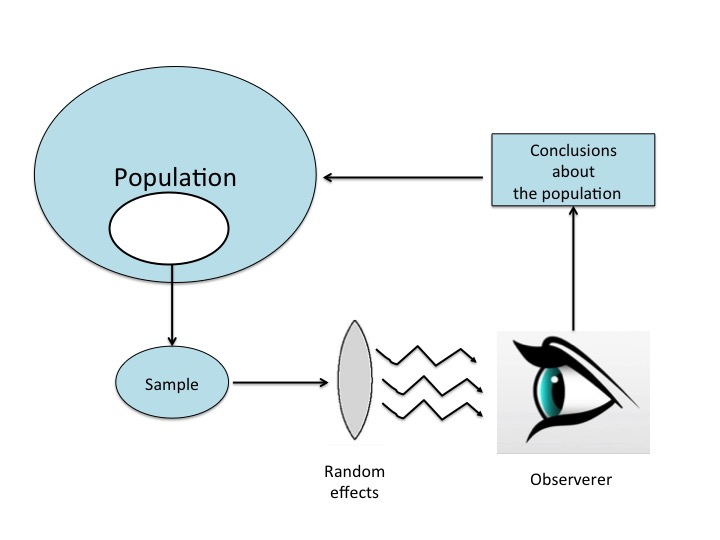
\includegraphics{_images/ExperimentalError.jpg}
\caption{Schematizzazione del processo sperimentale}
\end{figure}

In particolare, gli esperimenti debbono essere:

\begin{enumerate}
\def\labelenumi{\arabic{enumi}.}
\tightlist
\item
  Precisi
\item
  Accurati
\item
  Replicabili/Riproducibili
\end{enumerate}

In mancanza di questi requisiti, al termine dell'esperimento possono
rimanere dubbi sui risultati, tali da inficiare la validità delle
conclusioni raggiunte.

Forse vale la pena di chiarire cosa si intende con precisione,
accuratezza e replicabilità/riproducibilità. Abbiamo già visto che la
presenza dell'errore sperimentale ci impone di ripetere le misure più
volte. La precisione di un esperimento non è altro che la variabilità
dei risultati tra una replica e l'altra.

La precisione, da sola, non garantisce che l'esperimento sia affidabile.
Abbiamo menzionato nel capitolo precedente che l'errore sperimentale può
essere casuale o sistematico. Quest'ultimo può essere dovuto, per
esempio, ad uno strumento non accurato che sovrastima tutte le misure.
In questo caso, posso ripetere cento volte la misura, ottenendo sempre
lo stesso risultato, molto preciso, ma totalmente inaffidabile, nel
senso che non riflette la misura reale del soggetto. E'questa
l'accuratezza, cioè la capacità di una misura (o di un esperimento) di
restituire il valore reale, anche se dopo come media di numero molto
elevato di replicazioni.

L'accuratezza è molto più importante della precisione: infatti una
misura accurata, anche se imprecisa, riflette bene la realtà, anche se
in modo vago. Al contrario, una misura precisa ma inaccurata ci porta
completamente fuori strada, perchè non riflette la realtà! Un
esperimento/risultato non accurato si dice `distorto' (\emph{biased}).

Oltre a precisione ed accuratezza, siamo anche interessati alla
replicabilità di un esperimento, cioè alla possibilità che questo, se
ripetuto in condizioni assolutamente analoghe (stessi soggetti,
ambiente, strumenti\ldots{}) restituisca risultati equivalenti. Alcuni
biostatistici distinguono la replicabilità dalla riproducibilità, in
quanto considerano quest'ultima come la possibilità di ottenere
risultati equivalenti ripetendo una misura in condizioni diverse
(diversi soggetti, diverso ambiente\ldots{}). E'evidente che un
esperimento può essere totalmente accurato e replicabile, ma non
riproducibile con soggetti e condizioni ambientali diverse. Se è così,
le conclusioni raggiunte, anche se accurate, non possono essere
generalizzate.

\section{Elementi fondamentali del disegno
sperimentale}\label{elementi-fondamentali-del-disegno-sperimentale}

La metodica di organizzazione di un esperimento prende il nome di
\emph{disegno sperimentale} e deve essere sempre adeguatamente
formalizzata tramite la redazione di un \emph{protocollo sperimentale}
sufficientemente dettagliato da consentire a chiunque la replicazione
dell'esperimento e la verifica dei risultati.

Le basi del disegno sperimentale si fanno in genere risalire a Sir
Ronald A. Fisher, vissuto in Inghilterra dal 7 Febbraio 1890 al 29
luglio 1962. Laureatosi nel 1912, lavora come statistico per il comune
di Londra, fino a quando diviene socio della prestigiosa Eugenics
Education Society di Cambridge, fondata nel 1909 da Francis Galton,
cugino di Charles Darwin. Dopo la fine della guerra, Karl Pearson gli
propone un lavoro presso il rinomato Galton Laboratory, ma egli non
accetta a causa della profonda rivalità esistente tra lui e Pearson
stesso. Nel 1919 viene assunto presso la Rothamsted Experimental
Station, dove si occupa dell'elaborazione dei dati sperimentali e, nel
corso dei successivi 7 anni, definisce le basi del disegno sperimentale
ed elabora la sua teoria della ``analysis of variance''. Il suo libro
più importante è ``The design of experiment'', del 1935. E' sua la
definizione delle tre componenti fondamentali del disegno sperimentale:

\begin{enumerate}
\def\labelenumi{\arabic{enumi}.}
\tightlist
\item
  controllo degli errori;
\item
  replicazione;
\item
  randomizzazione.
\end{enumerate}

\subsection{Controllo degli errori}\label{controllo-degli-errori}

Controllare gli errori, o, analogamente, eseguire un esperimento
controllato signfica fondamentalmente due cose:

\begin{enumerate}
\def\labelenumi{\arabic{enumi}.}
\tightlist
\item
  adottare provvedimenti idonei ad evitare le fonti di errore,
  mantenendole al livello più basso possibile (alta precisione);
\item
  agire in modo da isolare l'effetto in studio (accuratezza), evitando
  che si confonda con effetti casuali e di altra natura.
\end{enumerate}

Declinare questi principi richiederebbe una vita di esperienza! Vogliamo
solo ricordare alcuni aspetti fondamentali.

\subsubsection{Campionamento corretto}\label{campionamento-corretto}

E'evidente che il primo requisito di un esperimento è una corretta
scelta delle unità sperimentali, cioè le più piccole unità che ricevono
lo `stimolo' rappresentato dal trattamento, in modo indipendente da
tutte le altre.

E' bene subito comprendere una fondamentale distinsione tra unità
sperimentali e unità osservazionali. Le prime sono appena state
definite; le seconde sono quelle che costituiscono l'oggetto della
misura e possono anche non coincidere con le prime. Ad esempio:
immaginiamo di trattare con un diserbante due vasetti, in modo
indipendente l'uno dall'altro. Immaginiamo poi di pesare singolarmente
le quattro piante di ciascun vasetto; in questa situazione, il vasetto è
l'unità sperimentale, le piante sono invece le unità osservazionali.
L'elemento discriminante di questo esempio è l'indipendenza: mentre le
unità sperimentali hanno ricevuto il trattamento in modo indipendente
l'una dall'altra, le unità osservazionali no. Questa differenza è
fondamentale, per motivi che vedremo più avanti.

Le unità sperimentali possono essere di varia natura; nel caso degli
esperimenti di campo, le unità sperimentali sono dette \textbf{parcelle}
e sono un pezzetto di terreno, di varia forma e dimensione.

\begin{figure}
\centering
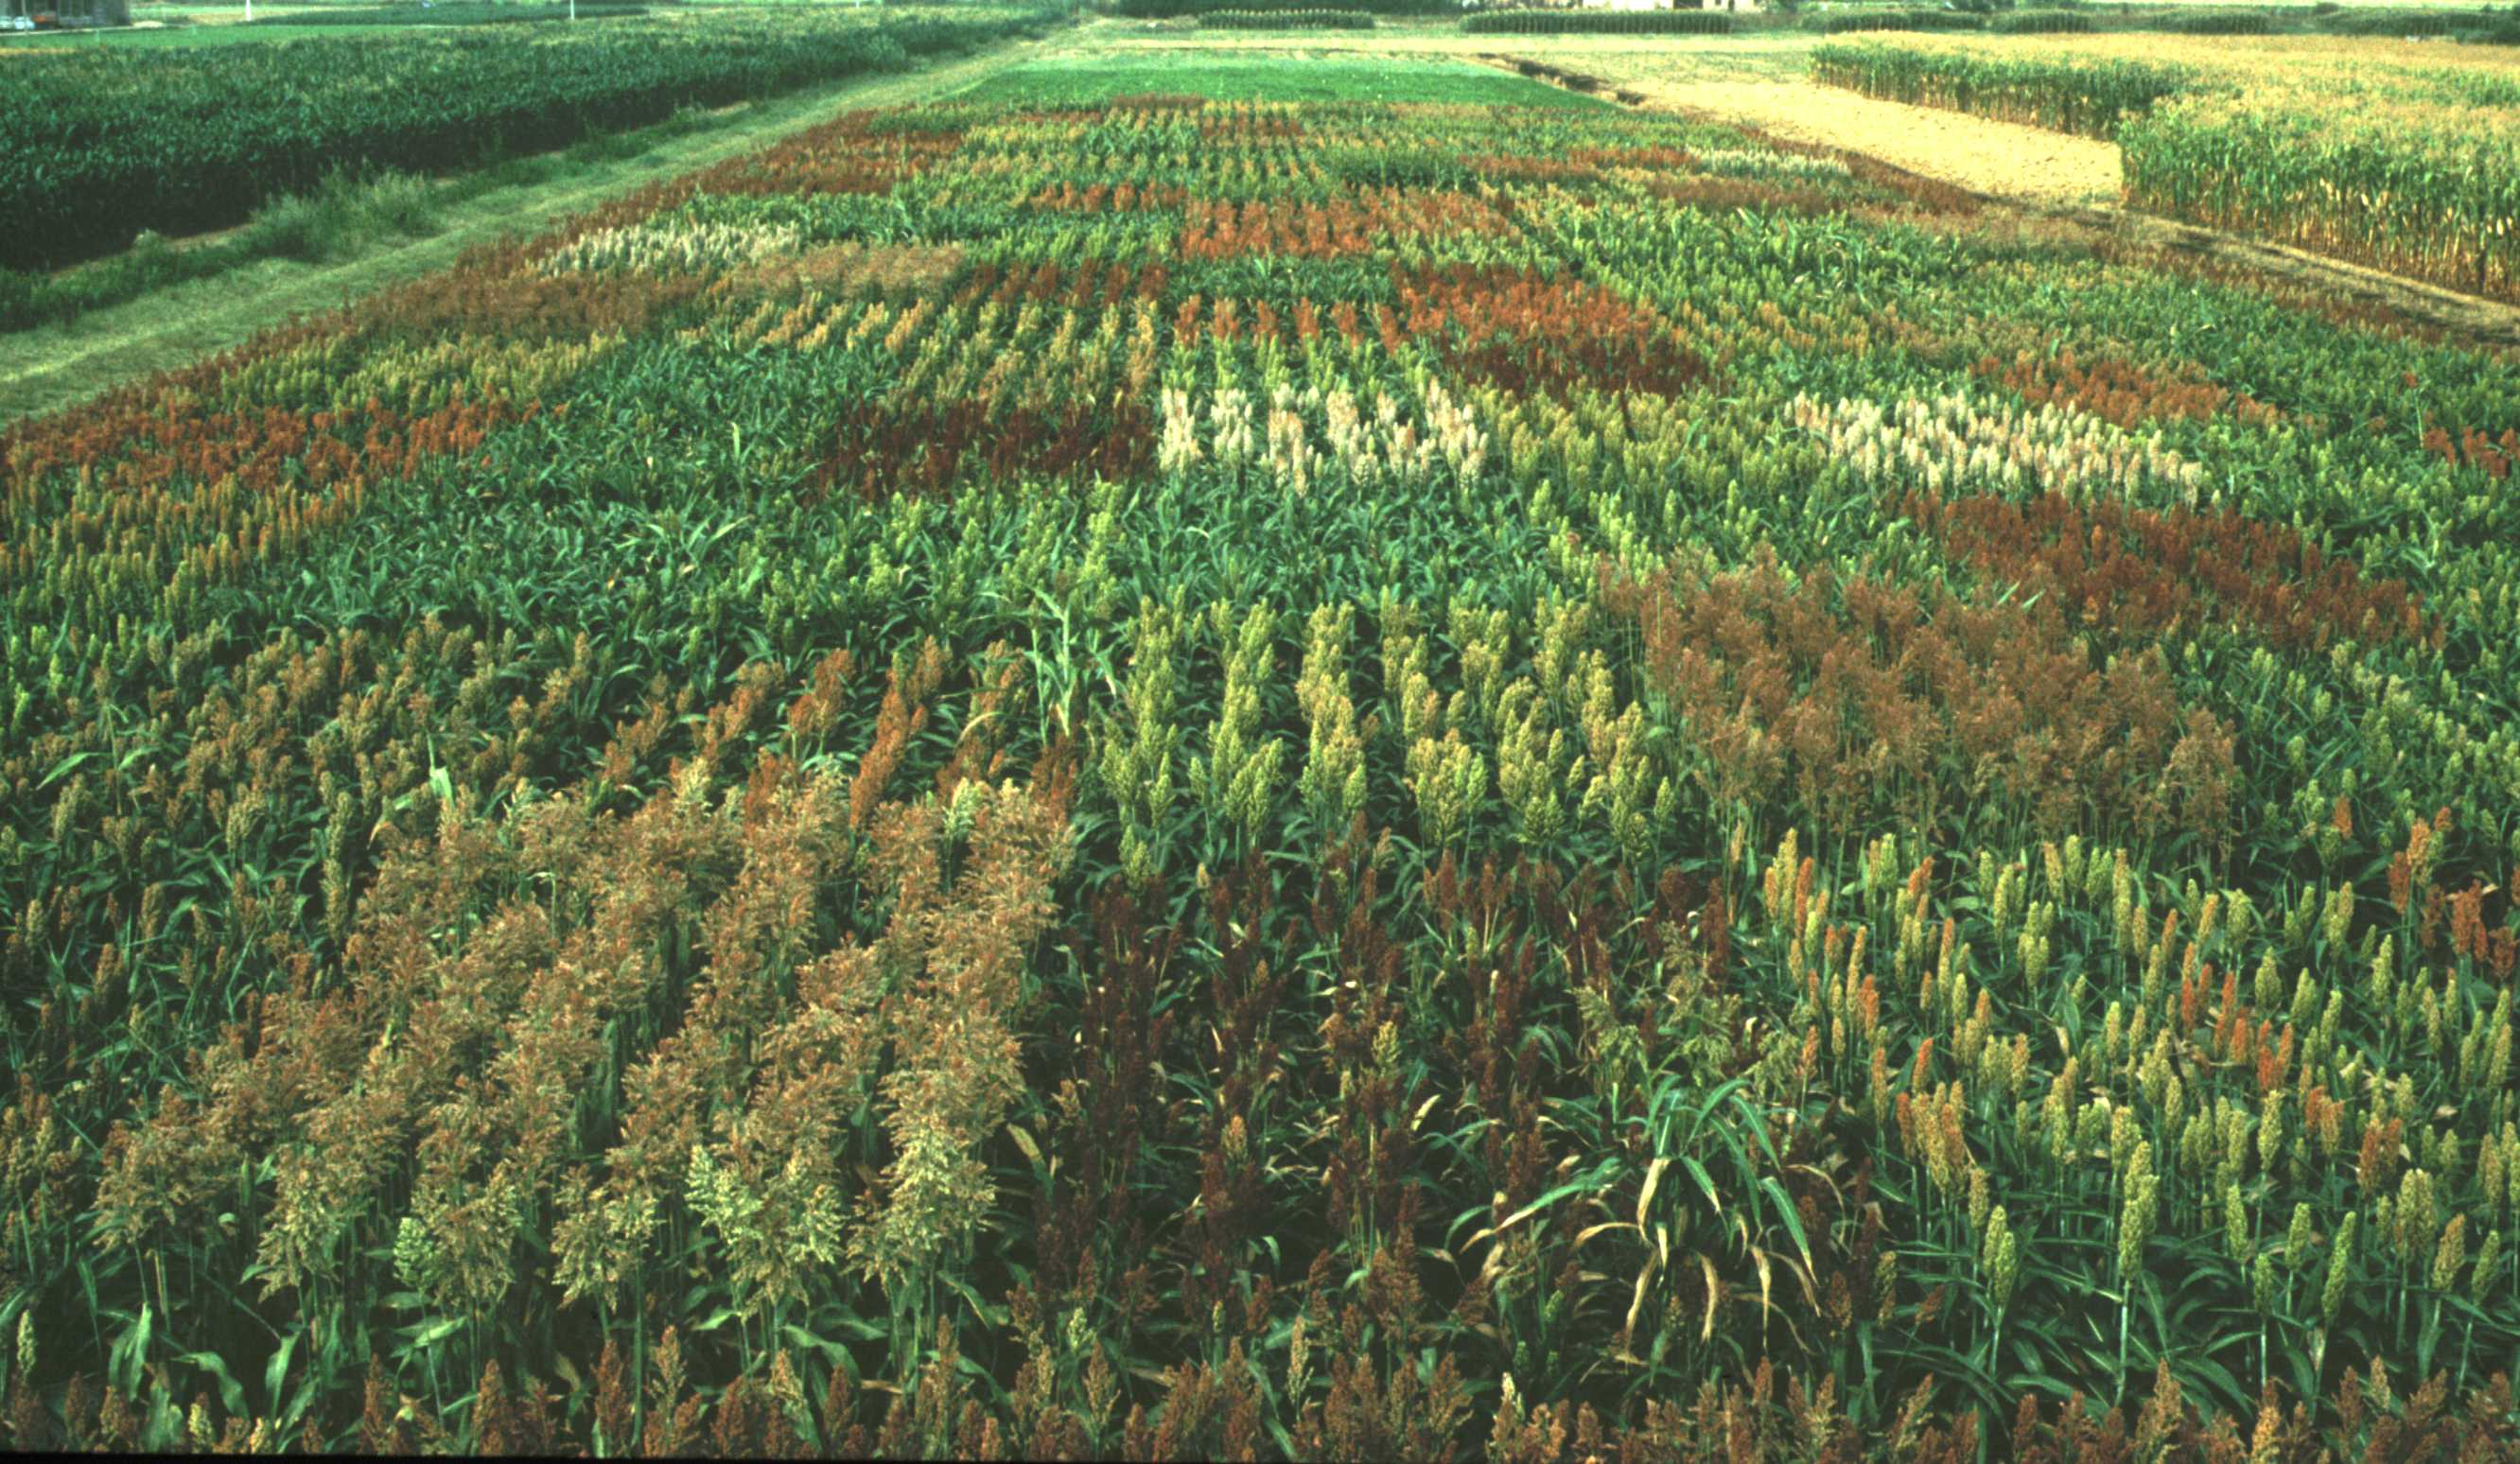
\includegraphics[width=0.90000\textwidth]{_images/SorgoProveVarietali.jpg}
\caption{Una prova sperimentale in campo (Foto D. Alberati)}
\end{figure}

Le unità sperimentali sono scelte per campionamento, che è un elemento
fondamentale dell'esperimento. Infatti, il censimento, che riguarda
tutti i soggetti di un certo ambito, non è, in se', un esperimento.
Ovviamente, il campione deve essere rappresentativo, altrimenti
l'esperimento è invalido.

Non è possibile dare indicazioni specifiche di campionamento, perché
queste dipendono dalla tipologia di esperimento. Illustriamo quindi solo
alcuni criteri generali.

Prima di campionare, dobbiamo avere una chiara visione della cornice di
campionamento, cioè della popolazione da cui io devo campionare. Devo
effettuare un esperimento valido per l'Italia centrale, per una località
particolare, per tutta Italia. Devo fare un esperimento che riguarda una
stalla in particolare o tutte le stalle dove si allevano bovini? Di
quale razza? E' un passaggio fondamentale, in quanto poi le conclusioni
non possono che riferirsi alla cornice della popolazione da cui il
campione è stato estratto, non altre. Per esperimenti nell'ambito delle
scienze sociali, diviene fondamentale che la cornice di campionamento
abbia le seguenti caratteristiche:

\begin{enumerate}
\def\labelenumi{\arabic{enumi}.}
\tightlist
\item
  le unità sono tutte identificabili e reperibili
\item
  le unità sono tutte caratterizzate (es. Id)
\item
  è aggiornata e organizzata logicamente
\item
  non mancano soggetti (che potrebbero quindi sfuggire al campionamento)
\item
  non ci sono soggetti duplicati
\item
  non ci sono elementi estranei
\end{enumerate}

Una volta che la popolazione è nota ed organizzata, dobbiamo trovare un
criterio di selezione. Fondamentalmente ci sono tre possibilità:

\begin{enumerate}
\def\labelenumi{\arabic{enumi}.}
\tightlist
\item
  campionamento randomizzato (casuale)
\item
  campionamento stratificato
\item
  campionamento sistematico
\end{enumerate}

Il campionamento randomizzato è tale che ogni soggetto ha la stessa
possibilità di ogni altro di essere incluso nel campione. Tipicamente,
questo campionamento è basato su un generatore di numeri casuali, con
distribuzione uniforme delle frequenze. Il codice sottostante serve per
ottenere cinque elementi casuali da un lotto di 48 identificati con
numeri progressivi.

\begin{Shaded}
\begin{Highlighting}[]
\KeywordTok{sample}\NormalTok{(}\DecValTok{1}\OperatorTok{:}\DecValTok{48}\NormalTok{, }\DecValTok{4}\NormalTok{)}
\end{Highlighting}
\end{Shaded}

\begin{verbatim}
## [1] 16 47 41 38
\end{verbatim}

Il campionamento casuale può non dare garanzie sufficienti di
rappresentatività. Per questo motivo, a volte, si utilizza il
\textbf{campionamento stratificato}, con il quale si divide la cornice
di campionamento in gruppi omogenei e si prelevano un certo numero di
soggetti da ogni gruppo. In questo caso è bene ricordare che potrebbe
essere auspicabile mantenere nel campione la stessa relazione tra gruppi
che esiste nella popolazione. Ad esempio, se in una popolazione di
insetti c'è il 10\% di maschi e il 90\% di femmine, io devo prelevare
\(n\) maschi e \(m\) femmine, tale che \(n/m = 0.1\), altrimenti il
campione che ottengo potrebbe non essere rappresentativo.

A volte, il campionamento può essere sistematico, nel senso che utilizzo
un criterio non casuale, ma in grado di assicurare una certa
rappresentatività. Ad esempio, per campionare gli edifici di una via,
potrei decidere di prendere il primo a caso e poi procedere prendendone
uno si e tre no. Questo campionamento è molto veloce e di facile
esecuzione, ma può dare origine a distorsioni.

Una forma di campionamento è quella a cluster: in questo caso suddivido
gli elementi in gruppi, scelgo a caso un certo numero di gruppi e poi
prendo tutti gli elementi di un gruppo. Ad esempio, devo selezionare i
bambini delle scuole elementari del comune di Perugia. In questo caso,
invece che selezionare i bambini, posso più velocemente selezionare le
scuole e prendere tutti i bambini delle scuole selezionate.
Evidentemente il metodo si basa sull'ipotesi che la selezione
rappresentativa delle scuole crea anche una selezione rappresentativa di
bambini.

A volte si esegue anche un campionamento a quota, cioè si prendono tutti
i soggetti che si incontrano in una certa situazione, fino a che non se
ne raccolgono un numero prefissato, per alcune classi specificate (Es.
30 donne, 25 uomini, 15 adolescenti e 20 bambini). Questo tipo di
campionamento è talvolta utilizzato negli esperimenti medici.

\subsubsection{Rigore}\label{rigore}

Direi che questo aspetto è ovvio e non richiede commenti particolari:
una ricerca deve essere condotta `a regola d'arte'. E' evidente che, ad
esempio, se vogliamo sapere la cinetica di degradazione di un erbicida a
20 °C dovremo realizzare una prova esattamente a quella temperatura, con
un erbicida uniformemente distribuito nel terreno, dentro una camera
climatica capace di un controllo perfetto della temperatura. Gli
strumenti dovranno essere ben tarati e sarà necessario attenersi
scrupolosamente a metodi validati e largamente condivisi.

Tuttavia, a proporsito di rigore, non bisogna scordare quanto diceva
C.F. Gauss a proposito della precisione nei calcoli, e che puà essere
anche riferito al rigore nella ricerca : ``\emph{Manca di mentalità
matematica tanto chi non sa riconoscere rapidamente ciò che è evidente,
quanto chi si attarda nei calcoli con una precisione superiore alla
necessità}''

\subsubsection{Omogeneità}\label{omogeneita}

Anche in questo caso, l'importanza di scegliere soggetti uniformi e
posti in un ambiente uniforme (nello spazio e nel tempo) è evidente.
Bisogna comunque tener presente che i risultati di un esperimento si
estendono alla popolazione da cui il campione è estratto e della quale
esso rappresenta le caratteristiche. Esperimenti nei quali si restringe
il campo di variabilità dei soggetti e dell'ambiente sono certamente più
precisi, ma forniscono anche risultati meno generalizzabili.
L'importante è avere ben chiaro su quale è il campo di validità che si
vuole dare ai risultati. Ad esempio, se si vuole ottenere un risultati
riferito alla collina umbra, bisognerà scegliere soggetti che
rappresentano bene la variabilità pedo-climatica della collina Umbra; né
più, né meno.

\subsubsection{\texorpdfstring{Evitare le `intrusioni
demoniache'}{Evitare le intrusioni demoniache}}\label{evitare-le-intrusioni-demoniache}

Secondo Hurlbert (1984), le intrusioni sono eventi totalmente casuali
che impattano negativamente con un esperimento in corso. E'evidente che,
ad esempio, un'alluvione, l'attacco di insetti o patogeni, la carenza
idrica hanno una pesante ricaduta sulla precisione di un esperimento e
sulla sua riuscita. Nello stesso lavoro, Hurlbert usa il termine
`intrusione demoniaca' per indicare quelle intrusioni che, pur casuali,
avrebbero potuto essere previste con un disegno più accurato,
sottolineando in questo caso la responsabilità dello sperimentatore.

Un esempio è questo: uno sperimentatore vuole studiare l'entità della
predazione dovuta alle volpi e quindi usa campi senza steccionate (dove
le volpi possono entrare) e campi protetti da steccionate (e quindi
liberi da volpi). Se le steccionate, essendo utilizzate dai falchi come
punto d'appoggio, finiscono per incrementare l'attività predatoria di
questi ultimi, si viene a creare un'intrusione demoniaca, che rende
l'esperimento distorto. Il demonio, in questo caso, non è il falco, che
danneggia l'esperimento, ma il ricercatore stesso, che non ha saputo
prevedere una possibile intrusione.

\subsection{Replicazione}\label{replicazione}

In ogni esperimento, i trattamenti dovrebbe essere replicati su 2 o più
unità sperimentali. Ciò permette di:

\begin{enumerate}
\def\labelenumi{\arabic{enumi}.}
\tightlist
\item
  dimostrare che i risultati sono replicabili (ma non è detto che siano
  riproducibili!)
\item
  rassicurare che eventuali circostanze aberranti casuali non abbiano
  provocati risultati distorti
\item
  misurare l'errore sperimentale, come variabilità di risposta tra
  repliche trattate nello stesso modo (precisione dell'esperimento)
\item
  incrementare la precisione dell'esperimento (più sono le repliche più
  l'esperimento è preciso, perchè si migliora la stima della
  caratteristica misurata, diminuendo l'incertezza)
\end{enumerate}

Per poter essere utili, le repliche debbono essere indipendenti, cioè
debbono \textbf{aver subito tutte le manipolazioni necessarie per
l'allocazione del trattamento in modo totalmente indipendente l'una
dall'altra}. Le manipolazioni comprendono tutte le pratiche necessarie,
come ad esempio la preparazione delle soluzioni, la diluizione dei
prodotti, ecc..

La manipolazione indipendente è fondamentale, perchè in ogni parte del
processo di trattamento possono nascondersi errori più o meno grandi,
che possono essere riconosciuti solo se colpiscono in modo casuale le
unità sperimentali. Se la manipolazione è, anche solo in parte, comune,
questi errori colpiscono tutte le repliche allo stesso modo, diventano
sistematici e quindi non più riconoscibili. Di conseguenza, si inficia
l'accuratezza dell'esperimento. Quando le repliche non sono
indipendenti, si parla di \textbf{pseudorepliche}, contrapposte alle
\textbf{repliche vere}.

Il numero di repliche dipende dal tipo di esperimento: più sono e meglio
è, anche se è necessario trovare un equilibrio accettabile tra
precisione e costo dell'esperimento. Nella sperimentazione di campo, 2
repliche sono poche, 3 appena sufficienti, 4 costituiscono la situazione
più comune, mentre un numero maggiore di repliche è abbastanza raro, non
solo per la difficoltà di seguire l'esperimento, ma anche perché
aumentano la dimensione della prova e, di conseguenza, la variabilità
del terreno.

\subsection{Randomizzazione}\label{randomizzazione}

L'indipendenza di manipolazione non garantisce da sola un esperimento
corretto. Infatti potrebbe accadere che le caratteristiche innate dei
soggetti, o una qualche `intrusione' influenzino in modo sistematico
tutte le unità sperimentali trattate nello stesso modo, così da
confondersi con l'effetto del trattamento. Un esempio banale è che
potremmo somministrare un farmaco a quattro soggetti in modo totalmente
indipendente, ma se i quattro soggetti fossero sistematicamente più alti
di quelli non trattati finiremmo per confondere una caratteristica
innata con l'effetto del farmaco. Oppure, se le repliche di un certo
trattamento si trovassero tutte vicine alla scolina, potrebbero essere
più danneggiate delle altre unità sperimentali dal ristagno idrico, il
cui effetto si confonderebbe con quello del trattamento stesso.

Questi problemi sono particolarmente insidiosi e si nascondono anche
dietro ai particolari apparentemente più insignificanti. La
randomizzazione è l'unico sistema per evitare, o almeno rendere molto
improbabile, la confusione dell'effetto del trattamento con fattori
casuali e/o comunque diversi dal trattamento stesso. La randomizzazione
si declina in vari modi:

\begin{enumerate}
\def\labelenumi{\arabic{enumi}.}
\tightlist
\item
  allocazione casuale del trattamento alle unità sperimentali. Gli
  esperimenti che prevedono l'allocazione del trattamento sono detti
  `manipolativi' o `disegnati'.
\item
  A volte l'allocazione del trattamento non è possibile o non è etica.
  Se volessimo studiare l'effetto delle cinture di sicurezza
  nell'evitare infortuni gravi, non potremmo certamente provocare
  incidenti deliberati. In questo caso la randomizzazione è legata alla
  scelta casuale di soggetti che sono `naturalmente' trattati.
  Esperimenti di questi tipo, si dicono \textbf{osservazionali}. Un
  esempio è la valutazione dell'effetto dell'inquinamento con metalli
  pesanti nella salute degli animali: ovviamente non è possibile, se non
  su piccola scala, realizzare il livello di inquinamento desiderato e,
  pertanto, dovremo scegliere soggetti che sono naturalmente sottoposti
  a questo genere di inquinamento, magari perché vivono vicino a zone
  industriali.
\item
  Se i soggetti sono immobili, la randomizzazione ha anche una
  connotazione legata alla disposizione spaziale e/o temporale casuale.
\end{enumerate}

L'assegnazione casuale del trattamento, o la selezione casuale dei
soggetti trattati, fanno si che tutti i soggetti abbiano la stessa
probabilità di ricevere qualunque trattamento oppure qualunque
intrusione casuale. In questo modo, la probabilità che tutte le repliche
di un trattamento abbiano qualche caratteristica innata o qualche
intrusione comune che li penalizzi/avvantaggi viene minimizzata. Di
conseguenza, confondere l'effetto del trattamento con variabilità
casuale (`confounding'), anche se teoricamente possibile, diviene
altamente improbabile.

\subsubsection{Gradienti e blocking}\label{gradienti-e-blocking}

Un esperimento in cui l'allocazione del trattamento, o la scelta dei
soggetti trattati, o la disposizione spaziale dei soggetti sono
totalmente casuali si dice `completamente randomizzato'. E'
perfettamente valido, perchè non pone dubbi fondati di inaccuratezza.
Tuttavia, in alcune circostanze è possibile porre restrizioni (vincoli)
alla randomizzazione, perchè ciò porta ad un esperimento più preciso.

In particolare, le unità sperimentali possono presentare delle
differenze, ad esempio di fertilità, oppure di sesso. Ad esempio,
randomizzare completamente l'allocazione dei trattamenti potrebbe far si
che tra le repliche di un trattamento vi siano più maschi che femmine,
il che crea un certo livello di `confounding'. Pertanto potrebbe essere
utile divider i soggetti in due gruppi (maschi e femmine), oppure in più
gruppi (molto fertile, mediamente fertile, poco fertile\ldots{}) e
randomizzare i trattamenti all'interno di ogni gruppo.

In generale, il \emph{blocking} consiste nel suddividere i soggetti in
gruppi uniformi e ripetere lo stesso esperimento (o parte di esso)
all'interno di ciascun gruppo, cioè in una situazione di maggiore
omogeneità.

Il raggruppamento delle unità sperimentali può tener conto di:

\begin{enumerate}
\def\labelenumi{\arabic{enumi}.}
\tightlist
\item
  vicinanza spaziale (campi, parcelle, stalle \ldots{})
\item
  caratteristiche fisiche (età, peso, sesso \ldots{} )
\item
  vicinanza temporale
\item
  gestione dei compiti (tecnico, valutatore, giudice \ldots{})
\end{enumerate}

Chiaramente, randomizzare all'interno del gruppo invece che randomizzare
completamente crea un vincolo. A volte i vincoli sono più di uno.
Vediamo un esempio. Una certa operazione industriale richiede un solo
operatore per essere portata a termine, ma può essere eseguita in
quattro modi diversi. Pianificate un esperimento per stabilire qual è il
metodo più veloce, avendo a disposizione solo quattro operatori.

L'unità sperimentale è il lavoratore. I metodi sono quattro e, volendo
lavorare con quattro repliche, avremmo bisogno di sedici operatori per
disegnare un esperimento completamente randomizzato. Possiamo tuttavia
considerare che un operatore, in quattro turni successivi, può operare
con tutti e quattro i metodi. Quindi possiamo disegnare un esperimento
in cui il turno fa da unità sperimentale e l'operatore fa da blocco
(blocchi randomizzati). Tuttavia, in ogni blocco (operatore) vi è un
gradiente, nel senso che i turni successivi al primo sono via via meno
efficienti, perché l'operatore accumula stanchezza. Per tener conto di
questo potremmo allora introdurre un vincolo ulteriore, per ogni
operatore, randomizzando i quattro metodi tra i turni, in modo che ogni
metodo, in operatori diversi, capiti in tutti i turni. In sostanza,
l'operatore fa da blocco, perché in esso sono contenuti tutti i metodi.
Ma anche il turno (per tutti gli operatori) fa da blocco, in quanto in
esso sono ancora contenuti tutti i metodi. Se non vi è chiaro, ci
torneremo sopra più tardi.

Posto che non si deve violare l'indipendenza delle repliche,
l'inclusione di vincoli alla randomizzazione è consentita, \textbf{ma
questa deve sempre essere tenuta presente in fase di analisi dei dati}.

Ronald Fisher diceva ``\emph{Analyse them as you have randomised
them}''. Meglio seguire il consiglio.

\subsubsection{E se ricercatori/soggetti sono
influenzabili?}\label{e-se-ricercatorisoggetti-sono-influenzabili}

Per concludere questa parte, è opportuno menzionare il fatto che, in un
esperimento scientifico, il fatto che lo sperimentatore e il soggetto
siano coscienti del trattamento somministrato può portare a risultati
distorti. Per esempio, nell'eseguire un rilievo, lo sperimentatore può
essere influenzato dal sapere con quale diserbante è stata trattata una
parcella, cercando inconsciamente conferme alle sue conoscenze
pregresse. D'altro canto, nei soggetti sperimentali dotati di coscienza
(uomo) sapere di essere stati trattati può influenzare l'esito del
trattamento (effetto placebo).

Per evitare questi problemi, soprattutto in ambito medico, un
esperimento può essere pianificato come:

\begin{enumerate}
\def\labelenumi{\arabic{enumi}.}
\tightlist
\item
  cieco: l'unità sperimentale o lo sperimentatore non sono coscienti dei
  dettagli del trattamento;
\item
  doppio cieco: né l'unità sperimentale né lo sperimentatore sono a
  coscienza dei dettagli del trattamento
\end{enumerate}

Un esperimento cieco e/o doppio cieco possono non essere eticamente
corretti oppure inutili, nel qual caso si torna ad un esperimento
tradizionale `aperto' (\emph{open experiment}: Tutti sanno tutto')

\subsection{Esperimenti non validi}\label{esperimenti-non-validi}

A questo punto dovrebbero essere chiare le caratteristiche di un
esperimento valido. A completamento, cerchiamo di elencare le
caratteristiche di un esperimento non valido.

\begin{enumerate}
\def\labelenumi{\arabic{enumi}.}
\tightlist
\item
  Cattivo controllo degli errori
\item
  Fondati sospetti di confounding
\item
  Mancanza di repliche vere
\item
  Confusione tra repliche vere e pseudo-repliche
\item
  Mancanza di randomizzazione
\item
  Presenza di vincoli alla randomizzazione, trascurati in fase di
  analisi.
\end{enumerate}

Le conseguenze di queste problematiche sono abbastanza diverse.

\subsubsection{Cattivo controllo degli
errori}\label{cattivo-controllo-degli-errori}

Bisogna verificare se il problema è relativo a questioni come la
mancanza di scrupolosità, l'uso di soggetti poco omogenei o di un
ambiente poco omogeneo, o altri aspetti che inficiano solo la
precisione, ma non l'accuratezza dell'esperimento. In questo caso,
l'esperimento è ancora valido (accurato), ma la bassa precisione
probabilmente impedirà di trarre conclusioni forti. Quindi, un
esperimento impreciso si `elimina' da solo, perché sarà inconclusivo. Di
questi esperimenti bisogna comunque diffidare, soprattutto quando siano
pianificati per mostrare l'assenza di differenze tra due trattamenti
alternativi. Mostrare l'assenza di differenze è facile: basta fare male
un esperimento, in modo che vi sia un alto livello di incertezza e
quindi l'evidenza scientifica sia molto debole.

Diversa è la situazione in cui un cattivo controllo degli errori, ad
esempio l'adozione di metodi sbagliati, porta a mancanza di accuratezza,
cioè a risultati che non riflettono la realtà (campionamento sbagliato,
ad esempio; oppure strumenti non tarati; impiego di metodi non validati
e/o non accettabili). In questo caso venendo a mancare l'accuratezza,
l'esperimento deve essere rigettato, in quanto non fornisce informazioni
realistiche.

\subsubsection{Confounding e correlazione
spuria}\label{confounding-e-correlazione-spuria}

Abbiamo appena menzionato il problema fondamentale della ricerca, cioè
il \textbf{confounding}, vale a dire la confusione tra l'effetto del
trattamento e un qualche altro effetto casuale, legato alle
caratteristiche innate del soggetto o a qualche intrusione più o meno
`demoniaca'. Abbiamo detto che non possiamo mai avere la certezza
dell'assenza di confounding, ma abbiamo anche detto che l'adozione di
una pratica sperimentale corretta ne minimizza la probabilità.

Chiaramente, rimangono dei rischi che sono tipici di situazioni nelle
quali il controllo adottato non è perfetto, come capita, ad esempio,
negli esperimenti osservazionali. In questo ambito è piuttosto temuta la
cosiddetta `correlazione spuria', una forma di confounding casuale per
cui due variabili variano congiuntamente (sono direttamente o
inversamente proporzionali), ma in modo del tutto casuale. Esistono, ad
esempio, dati che mostrano una chiara correlazione tra le vendite di
panna acida e le morti per incidenti in motocicletta. Chiaramente, non
esistono spiegazioni scientifiche per questo effetto, che è, ovviamente,
del tutto casuale. Il problema è che questa correlazione spuria non è
sempre così semplice da rintracciare.

\begin{figure}
\centering
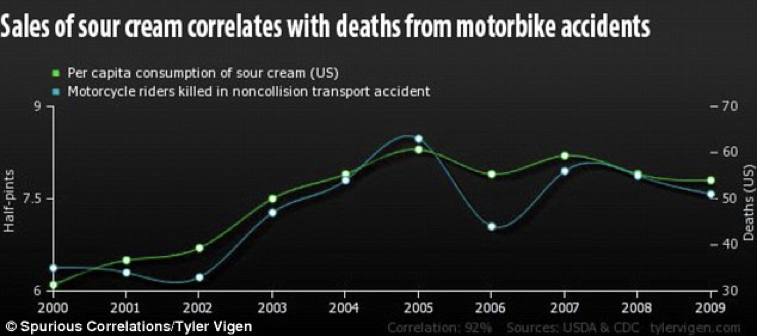
\includegraphics[width=0.90000\textwidth]{_images/PannaAcida.png}
\caption{Esempio di correlazione spuria}
\end{figure}

A volte il confounding non è casuale, ma è legato ad una variabile
esterna che si agisce all'insaputa dello sperimentatore. Ad esempio, è
stato osservato che il tasso di crimini è più alto nelle città che hanno
più chiese. La spiegazione di questo paradosso sta nel fatto che esiste
un `confounder', cioè l'ampiezza della popolazione. Nelle grandi città
si riscontrano sia una maggiore incidenza criminale, sia un grande
numero di chiese. In sostanza, la popolazione determina sia l'elevato
numero di chiese che l'elevato numero di crimini, ma queste ultime due
variabili non sono legate tra loro da una relazione causa-effetto (A
implica B e A implica C, ma B non implica C).

Il confounding non casuale è spesso difficile da evidenziare,
soprattutto se le correlazioni misurate sono spiegabili. Inoltre, non è
eliminabile con un'accurata randomizzazione, ma solo con l'esecuzione di
un esperimento totalmente controllato, nel quale ci si preoccupa di
rilevare tutte le variabili necessarie per spiegare gli effetti
riscontrati. Di questo è importante tener conto soprattutto negli
esperimenti osservazionali, dove il controllo è sempre più difficile e
meno completo.

\subsubsection{Pseudo-repliche e randomizzazione poco
attenta}\label{pseudo-repliche-e-randomizzazione-poco-attenta}

Per evidenziare questi problemi e comprendere meglio la differenza tra
un esperimento corretto e uno non corretto, è utilissima la
classificazione fatta da Hurlbert (1984), che riportiamo di seguito.

\begin{figure}
\centering
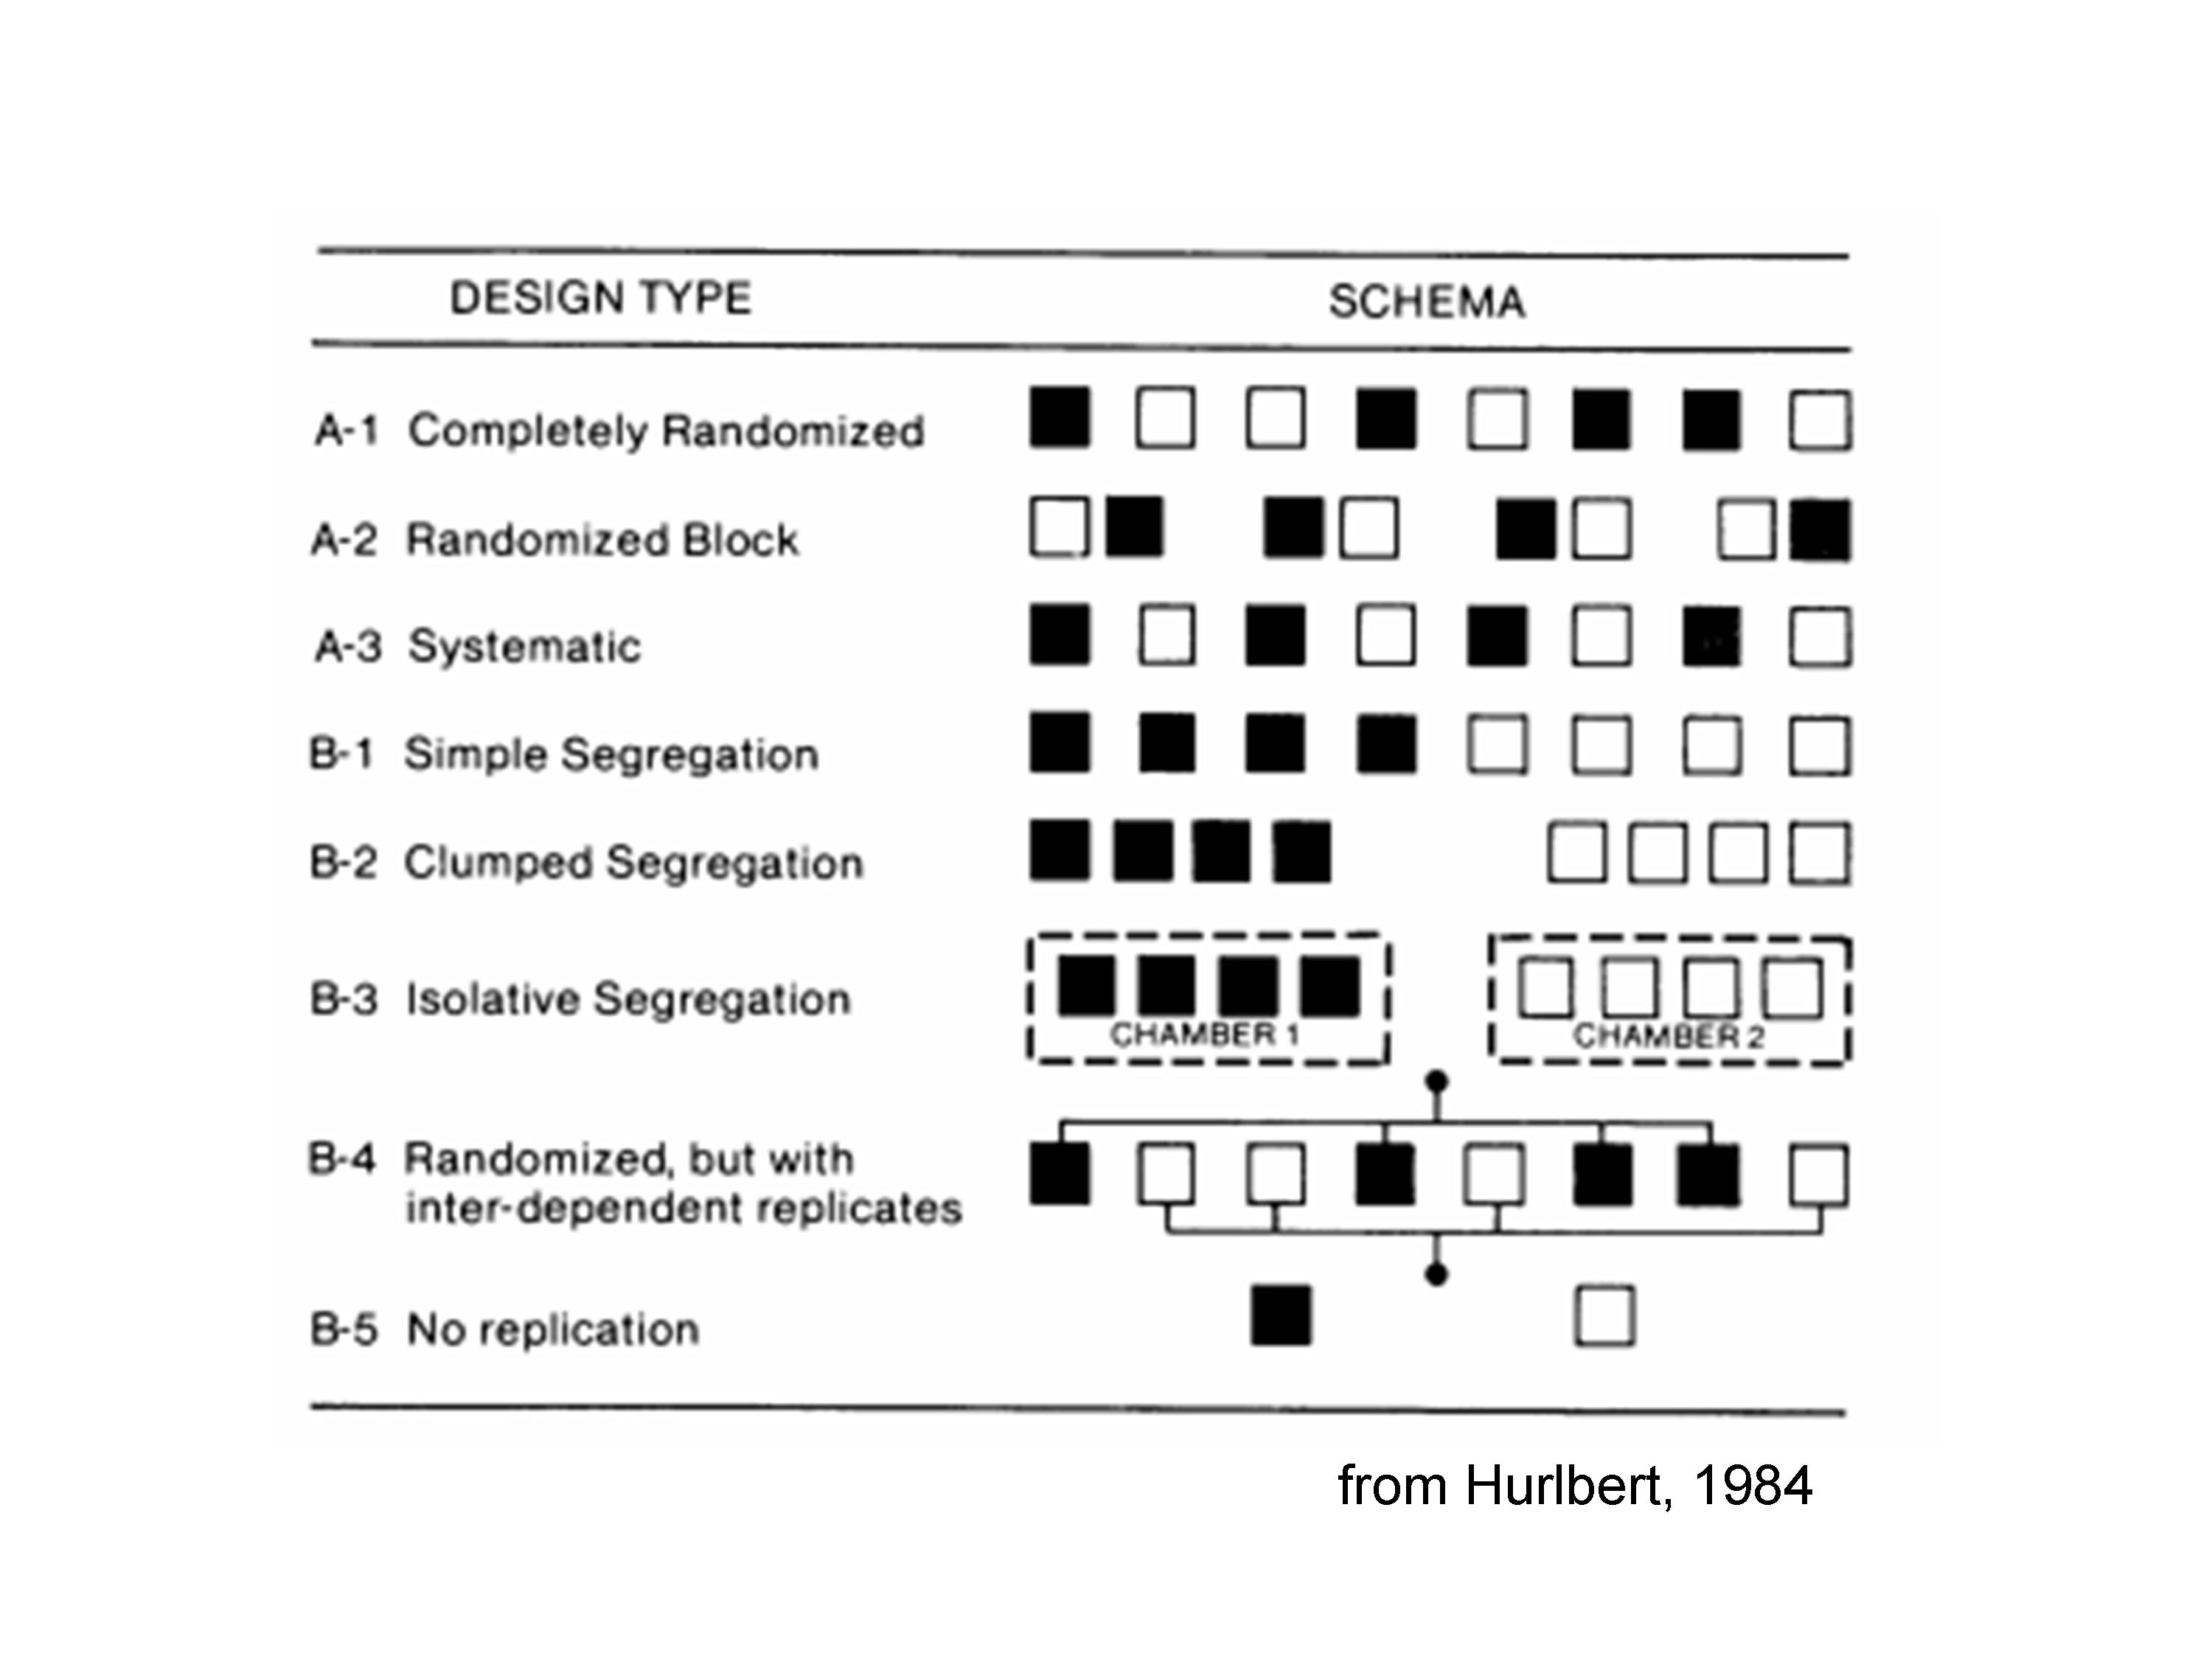
\includegraphics{_images/Randomisation.jpg}
\caption{Indicazioni per una corretta randomizzazione (Hurlbert, 1984)}
\end{figure}

Vengono mostrati 8 soggetti, sottoposti a due trattamenti (bianco e
nero), con 8 disegni sperimentali diversi.

Il disegno A1 è corretto, in quanto si tratta di un esperimento
completamente randomizzato. Ugualmente, è valido il disegno A2, nel
quale le unità sperimentali sono state divise in quattro gruppi omogenei
e sono state trattate in modo randomizzato all'interno di ogni gruppo.

Il disegno A3 è quantomeno `sospetto': vi sono repliche vere, ma
l'allocazione dei trattamenti non è randomizzata ed avviene con un
processo sistematico per il quale `nero' e `bianco' si alternano. Cosa
succederebbe se vi fosse un gradiente di fertilità decrescente da destra
verso sinistra? Le unità nere sarebbero avvantaggiate rispetto alle
bianche! Insomma, rimangono sospetti di confounding, a meno che non si
sia assolutamente certi dell'assenza di gradienti, come capita ad
esempio se all'interno dei blocchi, dobbiamo creare una sequenza
spazio-temporale. Vediamo tre esempi:

\begin{enumerate}
\def\labelenumi{\arabic{enumi}.}
\tightlist
\item
  ho quattro piante e, per ogni pianta, voglio confrontare un ramo basso
  con uno alto: è evidente che i due trattamenti sono sempre ordinati in
  modo sistematico (basso prima di alto).
\item
  Dobbiamo valutare l'effetto di fitofarmaci somministrati in due epoche
  diverse (accestimento e inizio-levata); anche qui non possiamo
  randomizzare, giacchè un'epoca precede sempre l'altra.
\item
  Dobbiamo confrontare la presenza di residui di un fitofarmaco a due
  profondità e non possiamo randomizzare, perché una profondità precede
  sempre l'altra nello spazio.
\end{enumerate}

In queste situazioni l'esperimento rimane valido, anche se la
randomizzazione segue un processo sistematico e non casuale.

Il disegno B1 è usualmente invalido: non vi è randomizzazione e ciò
massimizza i problemi del disegno A3: la separazione delle unità
sperimentali `bianche' e `nere' non consente una valutazione adeguata
dell'effetto del trattamento, che è confuso con ogni potenziale
differenza tra la parte destra e la sinistra dell'ambiente in cui la
sperimentazione viene eseguita. Ovviamente, la separazione può essere
non solo spaziale, ma anche temporale. Anche in questo caso diamo alcuni
esempi in cui una situazione come quella descritta in B1 è valida:

\begin{enumerate}
\def\labelenumi{\arabic{enumi}.}
\tightlist
\item
  Vogliamo confrontare la produzione in pianura e in collina. Ovviamente
  dobbiamo scegliere campioni in due situazioni fisicamente separate
\item
  Vogliamo confrontare la pescosità di due laghetti
\item
  Vogliamo confrontare la produttività di due campi contigui.
\end{enumerate}

Queste situazioni sono valide, anche se con una restrizione: non siamo
in grado di stabilire a chi debba essere attribuito l'effetto. Ad
esempio, per la prima situazione, pianura e collina possono dare
produzioni diverse per il suolo diverso, il clima diverso, la
precessione colturale diversa o un qualunque altro elemento che
differenzi le due località.

Il disegno B2 è analogo al disegno B1, ma il problema è più grave,
perché la separazione fisica è più evidente. Questo disegno è totalmente
sbagliato, a meno che non siamo specificatamente interessati all'effetto
località (vedi sopra).

Il disegno B3 è analogo al disegno B2, ma costituisce una situazione
molto frequente nella pratica scientifica. Immaginiamo infatti di voler
confrontare la germinazione dei semi a due temperature diverse,
utilizzando due camere climatiche e mettendo, in ognuna di esse, quattro
capsule Petri identiche. In questa situazione, l'effetto temperatura è
totalmente confuso con l'effetto `camera climatica (località)' e risente
di ogni malfunzionamente relativo ad una sola delle due camere. Inoltre,
le unità sperimentali con lo stesso trattamento di temperature non sono
manipolate in modo indipendente, dato che condividono la stessa camera
climatica. Di conseguenza, non si può parlare di repliche vere, bensì di
\textbf{pseudorepliche}.

Altri esempi di \textbf{pseudorepliche} sono schematizzati con il codice
B4. Ad esempio:

\begin{enumerate}
\def\labelenumi{\arabic{enumi}.}
\tightlist
\item
  trattare piante in vaso ed analizzare in modo indipendente i singoli
  individui invece che tutto il vaso;
\item
  trattare una parcella di terreno e prelevare da essa più campioni,
  analizzandoli separatamente;
\item
  trattare una capsula Petri ed analizzare separatamente i semi
  germinati al suo interno.
\end{enumerate}

Questi disegni, in assenza di repliche vere aggiuntive non sono da
considerarsi validi. Ad esempio, se io ho due vasetti trattati in modo
totalmente indipendente e da ciascuno di essi prelevo due piante e le
analizzo separatamente, il disegno è caratterizzato da due repliche vere
e due pseudorepliche per ogni replica ed è, pertanto, valido.

Il disegno B5 è invece evidentemente invalido, per totale mancanza di
repliche.

\begin{center}\rule{0.5\linewidth}{\linethickness}\end{center}

\section{Progettazione di un esperimento
(protocollo)}\label{progettazione-di-un-esperimento-protocollo}

Qualunque sia l'ambito scientifico, in ogni esperimento possiamo
individuare alcune fasi fondamentali, che proviamo ad elencare:

\begin{enumerate}
\def\labelenumi{\arabic{enumi}.}
\tightlist
\item
  Individuazione del background (ricerca bibliografica)
\item
  ipotesi scientifica;
\item
  definizione dell'obiettivo;
\item
  identificazione dei fattore/i sperimentale/i;
\item
  identificazione dei soggetti sperimentali e delle repliche;
\item
  identificazione delle variabili da rilevare;
\item
  allocazione randomizzata dei trattamenti (mappa dell'esperimento)
\item
  Esecuzione dell'esperimento
\end{enumerate}

Nell'analizzare questi aspetti, faremo riferimento ad alcuni esempi
pratici, che verranno indicati tra breve.

\subsection{\texorpdfstring{Ipotesi scientifica \(\rightarrow\)
obiettivo
dell'esperimento}{Ipotesi scientifica \textbackslash{}rightarrow obiettivo dell'esperimento}}\label{ipotesi-scientifica-rightarrow-obiettivo-dellesperimento}

Trascurando la parte di ricerca bibliografica, che è pur fondamentale,
nel metodo scientifico galileiano, il punto di partenza di un
esperimento è l'\textbf{ipotesi scientifica}, che determina l'obiettivo
dell'esperimento. Si tratta del passaggio fondamentale dal quale dipende
in modo logico tutto il lavoro successivo. Gli obiettivi debbono essere:

\begin{enumerate}
\def\labelenumi{\arabic{enumi}.}
\tightlist
\item
  rilevanti
\item
  chiaramente definiti;
\item
  specifici;
\item
  misurabili;
\item
  raggiungibili/realistici;
\item
  temporalmente organizzati.
\end{enumerate}

Il rischio che si corre con obiettivi mal posti è quello di eseguire una
ricerca dispersiva, con raccolta di dati non necessari e/o mancanza di
dati fondamentali, con costi più elevati del necessario e un uso poco
efficiente delle risorse. In genere, prima si definisce un obiettivo
generale, seguito da uno o più obiettivi specifici, in genere proiettati
su un più breve spazio temporale e che possono essere visti anche come
le fasi necessarie per raggiungere l'obiettivo generale.

Poniamo quattro esempi pratici.

\subsection{Casi di studio - 1}\label{casi-di-studio---1}

\subsubsection{Esempio 1 - Diserbo
chimico}\label{esempio-1---diserbo-chimico}

Si suppone che gli erbicidi A, B e C siano più efficaci di D, E ed F
verso \emph{Solanum nigrum}, una comune pianta infestante delle colture
di pomodoro. L'obiettivo generale della ricerca sarà quello di trovare
un'efficace soluzione per l'eliminazione di \emph{Solanum nigrum} dal
pomodoro. Gli obiettivi specifici saranno:

\begin{enumerate}
\def\labelenumi{\arabic{enumi}.}
\tightlist
\item
  valutare l'efficacia erbicida di A, B e C, confrontandola con quella
  di D, E ed F;
\item
  valutare la selettività degli anzidetti erbicidi verso il pomodoro;
\end{enumerate}

\subsubsection{Esempio 2 - Valutazione
varietale}\label{esempio-2---valutazione-varietale}

L'ipotesi è che le varietà di girasole A, B e C non hanno la stessa base
genetica e quindi non sono tutte ugualmente produttive. L'obiettivo
generale è quello di capire quale tra A, B e C sia più adatta alle
condizioni pedoclimatiche della collina Umbra.

Gli obiettivi specifici sono quelli di valutare:

\begin{enumerate}
\def\labelenumi{\arabic{enumi}.}
\tightlist
\item
  produttività di A, B e C
\item
  stabilità produttiva di A, B e C
\end{enumerate}

\subsubsection{Esempio 3 - Diserbo
parziale}\label{esempio-3---diserbo-parziale}

Nella barbabietola da zucchero, il diserbo localizzato lungo la fila
consente di diminuire l'impiego di erbicidi. Tuttavia, se la coltura
precedente ha prodotto semi e se non abbiamo effttuato una lavorazione
profonda per interrarli, la coltura sarà più infestata e quindi sarà più
difficile ottenere una buona produttività con il diserbo parziale.

Su questa ipotesi costruiamo un esperimento volto a valutare
l'interazione tra lavorazione del terreno e diserbo chimico. Per
raggiungere questo obiettivo generale, proveremo a valutare se:

\begin{enumerate}
\def\labelenumi{\arabic{enumi}.}
\tightlist
\item
  il diserbo parziale consente di ottenere produzioni comparabili a
  quelle del diserbo totale; 2.l'effetto è indipendente dalla
  lavorazione effettuata.
\end{enumerate}

\subsubsection{Esempio 4 - Colture
poliennali}\label{esempio-4---colture-poliennali}

L'ipotesi scientifica è affine a quella dell'esempio 2, ma, in questo
caso, vogliamo porre a confronto tre varietà di erba medica (A, B e C).
La differenza sta nel fatto che l'erba medica è una coltura poliennale e
quindi vogliamo capire se il giudizio di merito è indipendente dall'anno
di coltivazione.

I nostri obiettivi specifici saranno quindi:

\begin{enumerate}
\def\labelenumi{\arabic{enumi}.}
\tightlist
\item
  valutare la produttività media delle varietà in prova
\item
  valutare le oscillazione nei quattro anni di durata del cotico erboso
\end{enumerate}

\subsubsection{Esempio 5 - Inquinamento da
micotossine}\label{esempio-5---inquinamento-da-micotossine}

Secondo le notizie in bibliografia, i datteri confezionati in vendita
nei supermercati contengono elevate quantità di micotossine. L'obiettivo
generale è quello di verificare il livello di infestazione e vedere se
questo cambia con il metodo di confezionamento.

\begin{center}\rule{0.5\linewidth}{\linethickness}\end{center}

\subsection{Identificazione dei fattori
sperimentali}\label{identificazione-dei-fattori-sperimentali}

Dopo aver definito l'obiettivo di un esperimento, è necessario chiarire
esattamente gli stimoli a cui saranno sottoposte le unità sperimentali.
Uno `stimolo' sperimentale prende il nome di \textbf{fattore
sperimentale}, che può avere più \textbf{livelli}. I livelli del fattore
sperimentale prendono il nome di \textbf{trattamenti (o tesi)
sperimentali}.

\subsection{Esperimenti
(multi)fattoriali}\label{esperimenti-multifattoriali}

In alcuni casi è necessario inserire in prova più di un fattore
sperimentale. In questo caso si parla di esperimenti
\textbf{fattoriali}, che possono essere \textbf{incrociati (crossed)}
quando sono presenti in prova tutte le possibili combinazioni dei
livelli di ogni fattore, oppure di esperimenti \textbf{innestati
(nested)} quando i livelli di un fattore cambiano al cambiare dei
livelli dell'altro.

Ad esempio:

\begin{enumerate}
\def\labelenumi{\arabic{enumi}.}
\tightlist
\item
  Immaginiamo di voler studiare due fattori sperimentali: la varietà di
  girasole (tre livelli: A, B e C) e la concimazione (2 livelli: pollino
  e urea). Abbiamo quindi 6 possibili trattamenti (combinazioni):
  A-pollina, A-urea, B-pollina, B-urea, C-pollina e C-urea. Il disegno è
  completamente incrociato.
\item
  Immaginiamo di voler confrontare due specie in agricoltura biologica
  (orzo e triticale), con tre varietà ciascuna (A, B e C per orzo, D, E
  e F per triticale). Anche in questo caso abbiamo sei trattamenti:
  orzo-A, orzo-B, orzo-C, triticale-D, triticale-E e triticale-F, ma il
  disegno è innestato, perché per il fattore sperimentale `varietà' i
  livelli cambiano a seconda dei livelli del fattore `specie'.
\end{enumerate}

\subsection{Aggiungere un controllo?}\label{aggiungere-un-controllo}

In alcuni casi si pone il problema di inserire in prova un trattamento
che funga da riferimento per tutti gli altri. In questi casi si parla
comunemente di \textbf{controllo} o \textbf{testimone}, che può essere

\begin{itemize}
\tightlist
\item
  non sottosposto a trattamento
\item
  trattato con placebo
\item
  trattato secondo le modalità usuali di riferimento
\end{itemize}

\subsection{Fattori sperimentali di trattamento e di
blocco}\label{fattori-sperimentali-di-trattamento-e-di-blocco}

Finora abbiamo menzionato quelli che, in lingua inglese, vengono
definiti \emph{treatment factor} (trattamenti sperimentali). Tuttavia,
possono esserci altri fattori sperimentali non allocati, ma `innati' e
legati alla collocazione spazio-temporale o alle caratteristiche dei
soggetti. Questi fattori vengono definiti, sempre in inglese,
\emph{blocking factors}. Di questi fanno parte, ad esempio, il blocco,
la località ed ogni altro elemento che permette di raggruppare i
soggetti. Anche questi \emph{blocking factors} devono essere chiaramente
identificati ed elencati.

Su questa base identifichiamo i fattori sperimentali negli esempi
precedenti.

\subsection{Casi di studio - 2}\label{casi-di-studio---2}

\subsubsection{Esempio 1}\label{esempio-1}

Il fattore sperimentale oggetto di studio sarà il diserbo del pomodoro,
con 5 livelli inseriti in prova (6 trattamenti sperimentali): A, B, C,
D, E ed F. Inoltre, si ritiene opportuno inserire in prova un testimone
non trattato (NT), che ci permetterà di quantificare la percentuale di
malerbe controllate. Inoltre, sarà anche necessario inserire in prova un
testimone scerbato manualmente (ST), che ci permetterà di quantificare
eventuali perdite produttive dovute alla competizione residua o alla
fitotossicità del trattamento. In totale, avremo quindi 8 tesi
sperimentali. Come usuale in pieno campo, l'esperimento verrà disegnato
a blocchi randomizzati e sarà pertanto necessario inserire un fattore di
blocco.

\subsubsection{Esempio 2}\label{esempio-2}

Il fattore sperimentale in studio sarà la varietà di girasole con 3
livelli inclusi in prova (varietà A, B e C). Come testimone, inseriremo
la varietà di riferimento per la zona (D). Dato che eseguiremo questa
prova su un terreno nel quale vi sono due chiari gradienti di fertilità,
disegneremo l'esperimento considerando due fattori di blocco:
trasversale e longitudinale (spiego meglio tra poco\ldots{}). Poichè
dobbiamo valutare la stabilità produttiva, dovremo ripetere
l'esperimento più volte (es. in tre anni diversi) e quindi avremo un
secondo fattore sperimentale, incrociato con il primo.

\subsubsection{Esempio 3}\label{esempio-3}

In questo caso avremo due fattori sperimentali incrociati: il diserbo
con due livelli (totale o parziale, localizzato sulla fila) e la
lavorazione con tre livelli (aratura profonda, aratura superficiale e
\emph{minimum tillage}). Non vi è la necessità di un testimone, ma
avremo la necessità di un fattore di blocco. In totale, avremo sei tesi
sperimentali.

\subsubsection{Esempio 4}\label{esempio-4}

Il fattore sperimentale in studio sarà la varietà di erba medica con 3
livelli inclusi in prova (varietà A, B e C) ai quali aggiungiamo il
riferimento di zona (D) come testimone. Come nel caso del girasole,
dovremo valutare la stabilità produttiva negli anni, ma, dato che
abbiamo una coltura poliennale, non avremo bisogno di ripetere la prova,
ma potremo ripetere le osservazioni per quattro anni sulla stessa prova.

\subsubsection{Esempio 5}\label{esempio-5}

Per questo esperimento vengono considerate tre diverse modalità di
confezionamento (carta, busta di plastica, scatola di plastica
perforata). Non vi è necessità di un testimone, ma, dato che le diverse
confezioni verranno acquistate in diversi supermercati e dato che
sospettiamo differenze nella conservazione tra un supermercato e
l'altro, utilizzeremo il supermercato come fattore di raggruppamento.

\begin{center}\rule{0.5\linewidth}{\linethickness}\end{center}

\subsection{Identificazione delle unità sperimentali e delle
repliche}\label{identificazione-delle-unita-sperimentali-e-delle-repliche}

\subsubsection{Cornice di campionamento e numero di
repliche}\label{cornice-di-campionamento-e-numero-di-repliche}

Per i primi quattro esempi verranno eseguite prove di pieno campo, nella
Media Valle del Tevere, che rappresenta la cornice di campionamento
adeguata per l'obiettivo previsto. Sappiamo di dover selezionare
appezzamenti di terreno

\begin{enumerate}
\def\labelenumi{\arabic{enumi}.}
\tightlist
\item
  rappresentativi della Media Valle del Tevere,
\item
  omogenei.
\end{enumerate}

L'omogeneità dell'ambiente è fondamentale per aumentare la precisione
dell'esperimento. La scelta dell'appezzamento è chiaramente fondamentale
ed è guidata dall'esperienza, tenendo conto anche di aspetti come la
facilità di accesso e la vicinanza di strutture (laboratori,
capannoni\ldots{}) che consentano un'accurata esecuzione degli eventuali
prelievi.

Oltre alla scelta dell'appezzamento, si possono anche utilizzare alcune
strategie per favorire una buona omogeneità delle parcelle. Spesso si
usa far precedere la prova da una coltura di `omogeneizzazione', ad
esempio avena, che è molto avida di azoto e lascia nel terreno poca
fertilità residua. Oppure un prato di erba medica, che, grazie agli
sfalci periodici, lascia il terreno libero da piante infestanti.

Trattandosi di esperimenti di campo, il numero di repliche sarà di
quattro, per ogni trattamento e l'unità sperimentale sarà una parcella,
della quale dovremo valutare forma e dimensioni.

Per il quinto esempio, la cornice di campionamento sarà data dal
territorio del comune di Perugia. L'unità sperimentale sarà la
confezione e la scelta del numero di repliche dovrà essere compatibile
con la capacità di analisi per la determinazione dell'inquinamento da
micotossine. E' ragionevole pensare che 30 repliche (90 confezioni
totali) possano essere adeguate per rappresentatività e facilità di
gestione.

\subsubsection{Campionamento delle unità
sperimentali}\label{campionamento-delle-unita-sperimentali}

Per le quattro prove di pieno campo, una volta scelto l'appezzamento,
dovremo campionare le parcelle di terreno. Questa operazione viene
usualmente eseguita su carta, redigendo la \textbf{mappa
dell'esperimento}. In primo luogo, si decide la \textbf{dimensione e la
forma della parcella}.

L'aspetto fondamentale è che ogni parcella deve contenere un numero di
piante sufficientemente alto da essere rappresentativo. Per questo
motivo le colture a bassa fittezza hanno sempre bisogno di parcelle più
grandi che non quelle ad alta fittezza. La dimensione non deve tuttavia
eccedere una certa soglia, in quanto con essa aumenta anche la
variabilità del terreno e, di conseguenza, diminuisce l'omogeneità
dell'esperimento. Per questo motivo, talvolta si preferisce diminuire la
dimensione delle parcelle ed, avendo lo spazio sufficiente, aumentare il
numero delle repliche.

Nello stabilire la dimensione delle parcelle, dovremo tener conto del
fatto che la parte più delicata è il bordo, in quanto le piante che si
trovano lungo il bordo esterno risentono di condizioni diverse dalle
altre piante situate al centro della parcella (\textbf{effetto bordo}).
Questo determina variabilità all'interno della parcella, che possiamo
minimizzare raccogliendo solo la parte centrale. Si viene così a
distinguere la superficie totale della parcella dalla superficie di
raccolta (\textbf{superficie utile}), che può essere anche molto minore
di quella totale.

In generale si ritiene che le colture ad elevata fittezza (frumento,
cereali, erba medica\ldots{}) dovrebbero avere parcelle di almeno 10-20
\(m^2\), mentre a bassa fittezza (mis, girasole\ldots{}) dovrebbero
avere parcelle di almeno 20-40 \(m^2\). Queste dimensioni sono riferite
alla superficie utile di raccolta, non alla dimensione totale.

Per quanto riguarda la forma, le parcelle quadrate minimizzano l'effetto
bordo, perché, a parità di superficie, hanno un perimetro più basso.
Tuttavia esse sono di più difficile gestione, in quanto, considerando il
fronte di lavoro di una seminatrice o una mietitrebbiatrice parcellare,
possono richiedere la semina o la raccolta in più passate, il che
finisce per essere una fonte di errore. Per questo motivo le parcelle
sono usualmente rettangolari, con una larghezza pari a quella della
macchina impiegata per la semina.

Per i quattro esempi in studio potremmo utilizzare una dimensione delle
parcelle di 20 \(m^2\) per l'erba medica (2 m di larghezza per 10 m di
lunghezza) e di 22.5 \(m^2\) per pomodoro, mais e barbabietola da
zucchero (2.25 m di larghezza per 10 metri di lunghezza).

A questo punto possiamo redigere la mappa per il primo esempio. Dato che
il campo di prova è largo 30 metri e lungo 400 metri, potremmo
immaginare di disegnare otto file di percelle in senso trasversale (8 x
2.25m = 18m), di modo che l'esperimento non sia troppo lungo (il che ne
aumenterebbe la variabilità), ma rimanga spazio sufficiente ai lati, per
evitare di avvicinarsi troppo alle scoline, dove possono manifestarsi
ristagni idrici.

La mappa dell'esperimento è un elemento fondamentale e deve riportare
tutte le informazioni relative al disegno sperimentale. E'anche
importante indicare la direzione del Nord, in modo da facilitare
l'orientamento della mappa stessa. Notare inoltre che, intorno alla
prova, abbiamo sistemato altre parcelle fuori esperimento con funzione
di `bordi'. In questo modo si evita che i bordi esterni delle parcelle
esterne siano esposti a condizioni molto diverse dagli altri, cosa che
potrebbe accentuare l'effetto `bordo', di cui abbiamo parlato in
precedenza. Queste parcelle verranno trattate in modo ordinario (semina
e diserbo tradizionale del pomodoro).

\begin{figure}
\centering
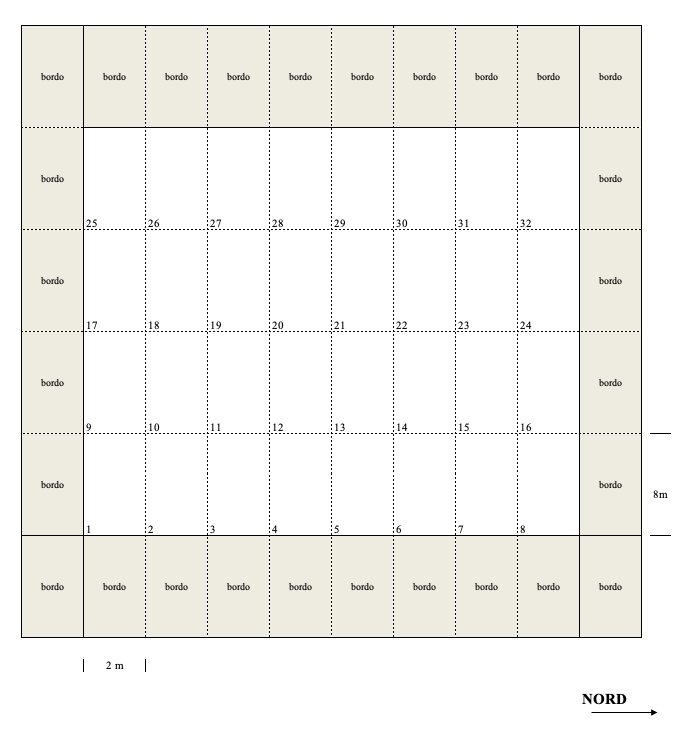
\includegraphics[width=0.90000\textwidth]{_images/Mappa1.png}
\caption{Mappa dell'esperimento relativo all esempio 1}
\end{figure}

Per l'esperimento relativo all'esempio 5, l'unità sperimentale è una
singola confezione di datteri, con le tipologie previste dal piano.

\begin{figure}
\centering
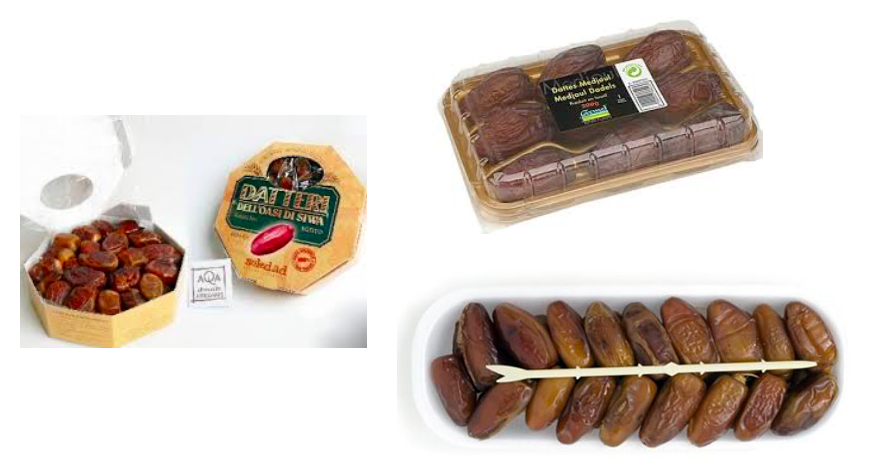
\includegraphics[width=0.90000\textwidth]{_images/Datteri.png}
\caption{Tipologie delle confezioni di datteri}
\end{figure}

Siccome è abbastanza scomodo campionare confezioni di datteri
casualmente all'interno del Comune di Perugia, si preferisce un
campionamento stratificato, selezionando 10 supermercati
rappresentativi, nelle zone più densamente popolate della città.
All'interno di ogni supermercato, si selezioneranno casualmente tre
repliche per ogni tipo di confezione.

\begin{center}\rule{0.5\linewidth}{\linethickness}\end{center}

\subsection{Scelta delle variabili da
rilevare}\label{scelta-delle-variabili-da-rilevare}

Durate e al termine dell'esperimento, sarà necessario rilevare le più
importanti caratteristiche dei soggetti sperimentali, sia quelle innate,
sia quelle indotte dai trattamenti sperimentali. Per ogni singolo
carattere, l'insieme delle modalità/valori che ognuno dei soggetti
presenta prende il nome di \textbf{variabile} (proprio perché varia,
cioè assume diversi valori, a seconda del soggetto). Ad esempio, quando
stiamo studiando l'effetto di due diserbanti su piante infestanti
appartenenti ad una certa specie, posto che l'unità sperimentale è
costituita da una singola pianta, possiamo avere le seguenti variabili:
il prodotto diserbante con cui ogni pianta è stata trattata, il peso di
ogni pianta prima del trattamento, il peso di ogni pianta dopo il
trattamento.

Le variabili sperimentali possono essere molto diverse tra di loro ed è
piuttosto importante saperle riconoscere, perché questo condiziona il
tipo di analisi statistica da eseguire.

\subsubsection{Variabili nominali
(categoriche)}\label{variabili-nominali-categoriche}

Le variabili nominali esprimono, per ciascun soggetto, l'appartenenza ad
una determinata categoria o raggruppamento. L'unica caratteristica delle
categorie è l'esclusività, cioè un soggetto che appartiene ad una di
esse non puà appartenere a nessuna delle altre. Variabili nominali sono,
ad esempio, il sesso, la varietà, il tipo di diserbante impiegato, la
modalità di lavorazione e così via. Le variabili categoriche permettono
di raggruppare i soggetti, ma non possono essere utilizzate per fare
calcoli, se non per definire le proporzioni dei soggetti in ciascun
gruppo.

\subsubsection{Variabili ordinali}\label{variabili-ordinali}

Anche le variabili ordinali esprimono, per ciascun soggetto,
l'appartenenza ad una determinata categoria o raggruppamento. Tuttavia,
le diverse categorie sono caratterizzate, oltre che dall'esclusività,
anche da una relazione di ordine, nel senso che è possibile stabilire
una naturale graduatoria tra esse. Ad esempio, la risposta degli
agricoltori a domande relative alla loro percezione sull'utilità di una
pratica agronomicapuò essere espressa utilizzando una scala con sei
categorie (0, 1, 2, 3, 4 e 5), in ordine crescente da 0 a 5. Di
conseguenza possiamo confrontare categorie diverse ed esprimere un
giudizio di ordine (2 è maggiore di 1, 3 è minore di 5), ma non possiamo
eseguire operazioni matematiche, tipo sottrarre dalla categoria 3 la
categoria 2 e così via, dato che la distanza tra le categorie non è
necessariamente la stessa.

\subsubsection{Variabili quantitative
discrete}\label{variabili-quantitative-discrete}

Le variabili discrete sono caratterizzate dal fatto che possiedono,
oltre alle proprietà dell'esclusività e dell'ordine, anche quella
dell'equidistanza tra gli attributi (es., in una scala a 5 punti, la
distanza -- o la differenza -- fra 1 e 3 è uguale a quella fra 2 e 4 e
doppia di quella tra 1 e 2). Le variabili discrete consentono la gran
parte delle operazioni matematiche e, spesso, possono essere analizzate
con metodiche parametriche, facendo riferimento alla distribuzione
normale, che, pur essendo continua, in alcune condizioni può essere
assunta come buona approssimazione di molte distribuzioni discrete.

\subsubsection{Variabili quantitative
continue}\label{variabili-quantitative-continue}

Le variabili quantitative continue possiedono tutte le proprietà
precedentemente esposte (esclusività delle categorie, ordine, distanza)
oltre alla continuità, almeno in un certo intervallo. Tipiche variabili
continue sono l'altezza, la produzione, il tempo, la fittezza\ldots{}

Dato che gli strumenti di misura nella realtà sono caratterizzati da una
certa risoluzione, si potrebbe arguire che misure su scala continua
effettivamente non esistono. Tuttavia questo argomento è più teorico che
pratico e, nella ricerca biologica, consideriamo continue tutte le
misure nelle quali la risoluzione dello strumento è sufficientemente
piccola rispetto alla grandezza da misurare. Viceversa, le variabili
continue sono piuttosto rare nelle scienze economiche e sociali in
genere.

La quantità di informazione fornita dagli strumenti di valutazione
cresce passando dalle scale nominali, di più basso livello, a quelle
quantitative continue, di livello più elevato. Variabili esprimibili con
scale quantitative continue o discrete possono essere espresse anche con
scale qualitative, adottando un'opportuna operazione di classamento. Il
contrario, cioè traformare in quantitativa una variabile qualitativa,
non è invece possibile.

\subsubsection{Rilievi visivi e
sensoriali}\label{rilievi-visivi-e-sensoriali}

Nella pratica sperimentale è molto frequente l'adozione di metodi di
rilievo basati sull'osservazione di un fenomeno attraverso uno dei sensi
(più spesso, la vista, ma anche gusto e olfatto) e l'assegnazione di una
valutazione su scala categorica, ordinale o, con un po' di prudenza,
quantitativa discreta o continua. Ad esempio, il ricoprimento delle
piante infestanti, la percentuale di controllo di un erbicida e la sua
fitotossicità vengono spesso rilevati visivamente, su scale da 0 a 100 o
simili.

I vantaggi di questa tecnica sono molteplici:

\begin{enumerate}
\def\labelenumi{\arabic{enumi}.}
\tightlist
\item
  Basso costo ed elevata velocità
\item
  Possibilità di tener conto di alcuni fattori perturbativi esterni, che
  sono esclusi dalla valutazione, contrariamente a quello che succede
  con metodi oggettivi di misura
\item
  non richiede strumentazione costosa
\end{enumerate}

A questi vantaggi fanno da contraltare alcuni svantaggi, cioè:

\begin{enumerate}
\def\labelenumi{\arabic{enumi}.}
\tightlist
\item
  Minor precisione (in generale)
\item
  Soggettività
\item
  L'osservatore può essere prevenuto
\item
  Difficoltà di mantenere uniformità di giudizio
\item
  Richiede esperienza specifica e allenamento
\end{enumerate}

I rilievi sensoriali sono ben accettati nella pratica scientifica in
alcuni ambiti ben definiti, anche se richiedono attenzione nell'analisi
dei dati non potendo essere assimilati \emph{tout court} con le misure
oggettive su scala continua.

\subsubsection{Variabili di
confondimento}\label{variabili-di-confondimento}

Quando si pianificano i rilievi da eseguire, oppure anche nel corso
dell'esecuzione di un esperimento, bisogna tener presente non soltanto
la variabile che esprime l'effetto del trattamento, ma anche tutte le
variabili che misurano possibili fattori di confondimento.

Ad esempio, immaginiamo di voler valutare la produttività di una specie
arborea in funzione della varietà. Immaginiamo anche di sapere che, per
questa specie, la produttività dipende anche dall'età. Se facciamo un
esperimento possiamo utilizzare alberi della stessa età per minimizzare
la variabilità dei soggetti. Tuttavia, se questo non fosse possibile,
per ogni albero dobbiamo rilevare non solo la produttività, ma anche
l'età, in modo da poter valutare anche l'effetto di questo fattore
aggiuntivo e separarlo dall'effetto della varietà. In questo modo
l'esperimento diviene molto più preciso.

\subsection{Casi di studio - 3}\label{casi-di-studio---3}

Per gli esempi in studio, immaginiamo per semplicità di dover rilevare
la produzione per gli esempi da 1 a 4 e il contenuto di micotossine per
l'esempio 5. Inoltre, per l'esempio 2, immaginiamo di dover rilevare
anche il peso di mille semi. Per questo, prenderemo dalla produzione di
granella di ogni parcella, quattro subcampioni da mille semi, da
sottoporre a successive misure.

\begin{center}\rule{0.5\linewidth}{\linethickness}\end{center}

\subsection{Allocazione dei
trattamenti}\label{allocazione-dei-trattamenti}

Il problema dell'allocazione dei trattamenti non si pone con l'esempio
5, in quanto, trattandosi di un esperimento osservazionale, le
confezione sono già `naturalmente' trattate, cioè appartengono già,
all'atto del campionamento, alla tipologia di confezionamento prescelta.

Per quanto riguarda gli altri esempi, abbiamo già redatto la mappa
secondo le necessità. A questo punto si pone il problema di decidere
quali parcelle trattare con cosa, nel rispetto dei trattamenti e delle
repliche prescelte. Per questo fine, semplici esperimentipossono anche
essere disegnati a mano; per esperimenti più complessi potremo
utilizzare il package \emph{agricolae} in R (de Mendiburu, 2017).

\subsection{Casi di studio - 4}\label{casi-di-studio---4}

\subsubsection{Esempio 1}\label{esempio-1-1}

Questo esempio va disegnato a blocchi randomizzati; tuttavia, a titolo
di esempio, esamineremo anche la possibilità che venga disegnato a
randomizzazione completa. Quest'ultimo disegno è il più semplice e
consiste nell'assegnare ogni trattamento a quattro parcelle casualmente
scelte. Con R bisognerà prima creare il vettore dei nomi delle tesi e il
numero di repliche per tesi

\begin{Shaded}
\begin{Highlighting}[]
\KeywordTok{library}\NormalTok{(agricolae)}
\NormalTok{trt <-}\StringTok{ }\KeywordTok{c}\NormalTok{(}\StringTok{"A"}\NormalTok{, }\StringTok{"B"}\NormalTok{, }\StringTok{"C"}\NormalTok{, }\StringTok{"D"}\NormalTok{, }\StringTok{"E"}\NormalTok{, }\StringTok{"F"}\NormalTok{, }\StringTok{"NT"}\NormalTok{, }\StringTok{"TS"}\NormalTok{)}
\NormalTok{reps <-}\StringTok{ }\KeywordTok{rep}\NormalTok{(}\DecValTok{4}\NormalTok{, }\DecValTok{8}\NormalTok{)}
\NormalTok{design <-}\StringTok{ }\KeywordTok{design.crd}\NormalTok{(trt, }\DataTypeTok{r=}\NormalTok{reps, }\DataTypeTok{seed=}\DecValTok{777}\NormalTok{, }\DataTypeTok{serie=}\DecValTok{0}\NormalTok{)}
\NormalTok{design}\OperatorTok{$}\NormalTok{book}
\end{Highlighting}
\end{Shaded}

\begin{verbatim}
##    plots r trt
## 1      1 1   E
## 2      2 1   C
## 3      3 1   B
## 4      4 2   C
## 5      5 1   F
## 6      6 1  TS
## 7      7 1  NT
## 8      8 1   D
## 9      9 2  NT
## 10    10 1   A
## 11    11 2  TS
## 12    12 2   F
## 13    13 3  NT
## 14    14 3   C
## 15    15 3  TS
## 16    16 2   D
## 17    17 3   D
## 18    18 2   E
## 19    19 3   E
## 20    20 4  NT
## 21    21 2   A
## 22    22 4   D
## 23    23 4   E
## 24    24 3   A
## 25    25 4   C
## 26    26 2   B
## 27    27 4   A
## 28    28 3   F
## 29    29 3   B
## 30    30 4  TS
## 31    31 4   F
## 32    32 4   B
\end{verbatim}

Possiamo ora riportare la randomizzazione sulla mappa disegnata in
precedenza.

\begin{figure}
\centering
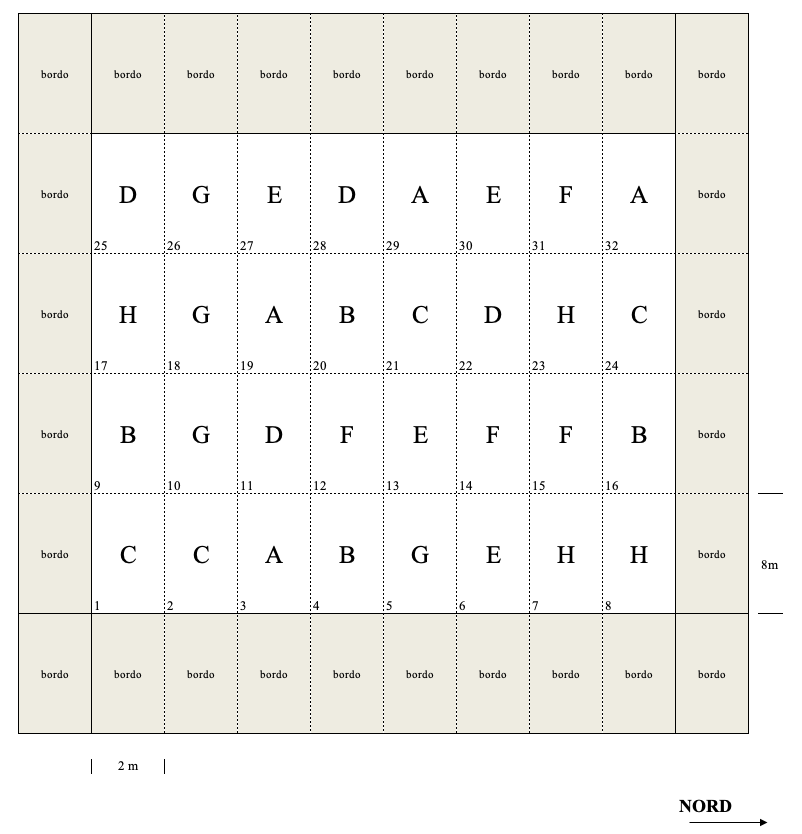
\includegraphics[width=0.90000\textwidth]{_images/Mappa1CRD.png}
\caption{Schema sperimentale a randomizzazione completa per l'Esempio 1}
\end{figure}

Questo schema è eccellente se l'ambiente è molto uniforme. Tuttavia, nel
caso di un esperimento di camp è lecito aspettarsi un gradiente
trasversale, dato che il campo sarà certamente meno fertile vicino alle
scoline. Per questo motivo disegneremo l'esperimento a blocchi
randomizzati, dividendo prima l'appezzamento in quattro blocchi
perpendicolari al gradiente di fertilità. Ad esempio il blocco 1
conterrà le parcelle 1, 9, 17, 25 2, 10, 18 e 26, cioè le prime due
colonne della mappa, con un numero di parcellè esattamente uguali al
numero delle tesi. Il blocco 2 conterrà le colonne 3 e 4 e così via.
Dato che il gradiente è trasversale, le parcelle di un stesso blocco
saranno più omogenee che non parcelle su blocchi diversi. Dopo aver
diviso la mappa in quattro blocchi di otto parcelle, possiamo allocare
gli otto trattamenti a random all'interno di ogni blocco. Con R è
possibile utilizzare il codice seguente (notare che la numerazione
assegnata da R è diversa dalla nostra, anche se possiamo far riferimento
ai valori crescenti all'interno di ogni blocco).

\begin{Shaded}
\begin{Highlighting}[]
\NormalTok{reps <-}\StringTok{ }\DecValTok{4}
\NormalTok{designRCBD <-}\StringTok{ }\KeywordTok{design.rcbd}\NormalTok{(trt, }\DataTypeTok{r=}\NormalTok{reps, }\DataTypeTok{seed=}\DecValTok{777}\NormalTok{, }\DataTypeTok{serie=}\DecValTok{2}\NormalTok{)}
\NormalTok{book2 <-}\StringTok{ }\NormalTok{designRCBD}\OperatorTok{$}\NormalTok{book}
\NormalTok{book2}
\end{Highlighting}
\end{Shaded}

\begin{verbatim}
##    plots block trt
## 1    101     1   E
## 2    102     1   B
## 3    103     1  NT
## 4    104     1   F
## 5    105     1   D
## 6    106     1  TS
## 7    107     1   C
## 8    108     1   A
## 9    201     2   F
## 10   202     2   A
## 11   203     2   C
## 12   204     2   E
## 13   205     2  TS
## 14   206     2   B
## 15   207     2  NT
## 16   208     2   D
## 17   301     3  TS
## 18   302     3  NT
## 19   303     3   F
## 20   304     3   A
## 21   305     3   B
## 22   306     3   E
## 23   307     3   C
## 24   308     3   D
## 25   401     4   D
## 26   402     4  TS
## 27   403     4   A
## 28   404     4   F
## 29   405     4   E
## 30   406     4   C
## 31   407     4   B
## 32   408     4  NT
\end{verbatim}

\begin{Shaded}
\begin{Highlighting}[]
\KeywordTok{zigzag}\NormalTok{(designRCBD) }\CommentTok{# zigzag numeration}
\end{Highlighting}
\end{Shaded}

\begin{verbatim}
##    plots block trt
## 1    101     1   E
## 2    102     1   B
## 3    103     1  NT
## 4    104     1   F
## 5    105     1   D
## 6    106     1  TS
## 7    107     1   C
## 8    108     1   A
## 9    208     2   F
## 10   207     2   A
## 11   206     2   C
## 12   205     2   E
## 13   204     2  TS
## 14   203     2   B
## 15   202     2  NT
## 16   201     2   D
## 17   301     3  TS
## 18   302     3  NT
## 19   303     3   F
## 20   304     3   A
## 21   305     3   B
## 22   306     3   E
## 23   307     3   C
## 24   308     3   D
## 25   408     4   D
## 26   407     4  TS
## 27   406     4   A
## 28   405     4   F
## 29   404     4   E
## 30   403     4   C
## 31   402     4   B
## 32   401     4  NT
\end{verbatim}

\begin{Shaded}
\begin{Highlighting}[]
\KeywordTok{print}\NormalTok{(designRCBD}\OperatorTok{$}\NormalTok{sketch)}
\end{Highlighting}
\end{Shaded}

\begin{verbatim}
##      [,1] [,2] [,3] [,4] [,5] [,6] [,7] [,8]
## [1,] "E"  "B"  "NT" "F"  "D"  "TS" "C"  "A" 
## [2,] "F"  "A"  "C"  "E"  "TS" "B"  "NT" "D" 
## [3,] "TS" "NT" "F"  "A"  "B"  "E"  "C"  "D" 
## [4,] "D"  "TS" "A"  "F"  "E"  "C"  "B"  "NT"
\end{verbatim}

Anche in questo caso, riportiamo tutto sulla mappa.

\begin{figure}
\centering
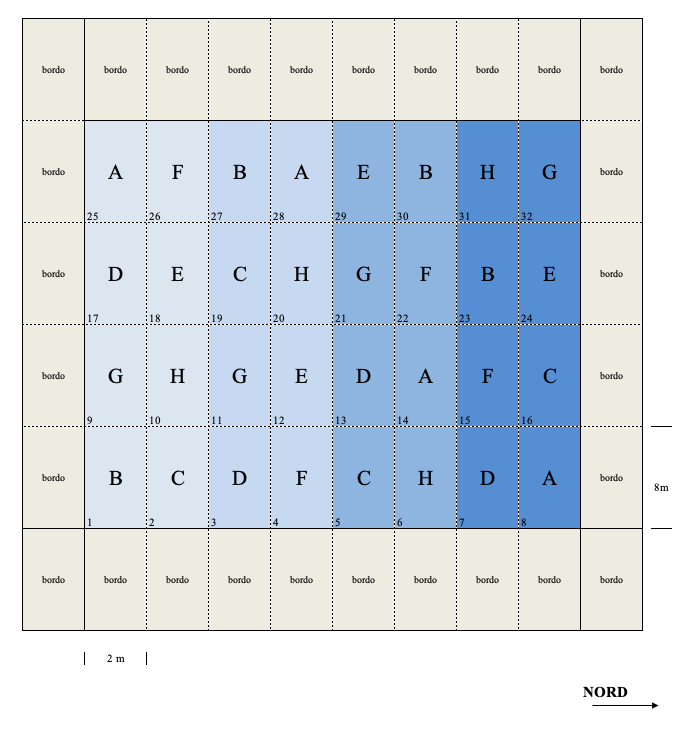
\includegraphics[width=0.90000\textwidth]{_images/Mappa1CRBD.png}
\caption{Schema sperimentale a blocchi randomizzati per l'Esempio 1}
\end{figure}

\subsubsection{Esempio 2}\label{esempio-2-1}

In questo caso, per ognuno dei tre anni di prova, la mappa contiene una
griglia 4 x 4, analoga a quella dell'esperimento precedente, ma più
piccola. Nella mappa potremo quindi identificare, esclusi i bordi,
quattro colonne e quattro righe. Dato che abbiamo presupposto
l'esistenza di un gradiente trasversale e lungitudinale (tra righe e tra
colonne), l'allocazione dei trattamenti dovrà esser fatta in modo che
ognuno di essi si trovi su ogni riga e ogni colonna. Questo tipo di
disegno prende il nome di \textbf{Quadrato latino}.

Anche in questo caso potremo chiedere ad R di aiutarci a trovare la
combinazione corretta (anche se questo potrebbe essere comodamente fatto
a mano).

\begin{Shaded}
\begin{Highlighting}[]
\NormalTok{trt <-}\StringTok{ }\KeywordTok{c}\NormalTok{(}\StringTok{"A"}\NormalTok{, }\StringTok{"B"}\NormalTok{, }\StringTok{"C"}\NormalTok{, }\StringTok{"D"}\NormalTok{)}
\NormalTok{designLS <-}\StringTok{ }\KeywordTok{design.lsd}\NormalTok{(trt, }\DataTypeTok{seed=}\DecValTok{543}\NormalTok{, }\DataTypeTok{serie=}\DecValTok{2}\NormalTok{)}
\NormalTok{designLS}\OperatorTok{$}\NormalTok{book}
\end{Highlighting}
\end{Shaded}

\begin{verbatim}
##    plots row col trt
## 1    101   1   1   C
## 2    102   1   2   A
## 3    103   1   3   B
## 4    104   1   4   D
## 5    201   2   1   D
## 6    202   2   2   B
## 7    203   2   3   C
## 8    204   2   4   A
## 9    301   3   1   B
## 10   302   3   2   D
## 11   303   3   3   A
## 12   304   3   4   C
## 13   401   4   1   A
## 14   402   4   2   C
## 15   403   4   3   D
## 16   404   4   4   B
\end{verbatim}

\begin{figure}
\centering
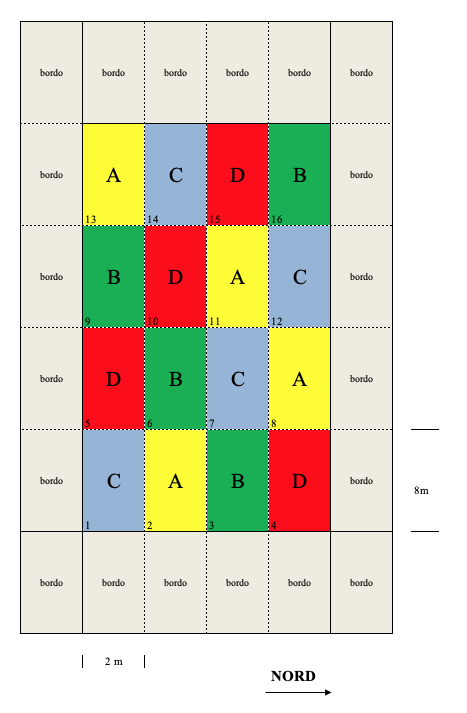
\includegraphics[width=0.90000\textwidth]{_images/Mappa2LS.png}
\caption{Schema sperimentale a quadrato latino per l'Esempio 2 (un
anno)}
\end{figure}

A questo punto dobbiamo considerare che questa prova deve essere
ripetuta in tre anni. La ripetizione di una prova è sempre fondamentale,
in quanto consente di verificare non solo la replicabilità
dell'esperimento (che è dimostrata dalle repliche), ma anche la sua
riproducibilità (riguardare le definizioni di replicabilità e
riproducibilità). In questo caso poi la ripetizione dell'esperimento è
indispensabile per misurare la stabilità produttiva, cioè l'oscillazione
delle produzioni da un anno all'altro.

Ovviamente è anche importante verificare la stabilità produttiva da una
località all'altra, che consente di valutare l'esistenza di
macro-areali, nei quali è possibile consigliare le stesse varietà.
Un'aspetto fondamentale è comunque quello di \textbf{definire una
diversa randomizzazione in ogni anno/località}, per evitare che le
stesse varietà siano sempre nelle stesse posizioni, che potrebbe dare
origine a dubbi di confounding. La definizione delle randomizzazioni per
il secondo e terzo anno è lasciata per esercizio.

Un'altro aspetto da considerare è la metodica impiegata per la
determinazione del peso di 1000 semi. Abbiamo già visto che, per
aumentare la precisione e la rappresentatività, da tutta la granella
raccolta da una parcella preleviamo quattro lotti da 1000 semi, di cui
determinare il peso. In questo modo, per ogni trattamento avremo 16
valori (quattro repliche x quattro lotti per replica). Ovviamente non
possiamo affermare di avere 16 repliche, in quanto solo le parcelle sono
da considerare repliche, in quanto ricevono il trattamento (varietà) in
modo indipendente. I quattro lotti raccolti da ogni parcella sono unità
osservazionali (perché ne viene rilevato il peso), ma non unità
sperimentali, perché appartengono alla stessa parcella e non sono
indipendenti. I quattro lotti si dicono \textbf{sub-repliche}, quindi il
disegno ha quattro repliche e quattro sub-repliche per replica
(\textbf{disegno a quadrato latino con sottocampionamento}). I due
strati di errore (variabilità tra repliche e variabilità tra
sub-repliche entro replica), devono essere mantenuti separati in fase di
analisi, altrimenti l'analisi è invalida, perché è condotta come se
avessimo un più alto grado di precisione (16 repliche) rispetto a quello
che abbiamo effettivamente (una sorta di millantato credito!).

\subsubsection{Esempio 3}\label{esempio-3-1}

In questo caso abbiamo un disegno fattoriale con due livelli a blocchi
randomizzati. Nel principio, questo disegno non ha nulla di diverso da
quello relativo all'esempio 1, fatto salvo un minor numero di
trattamenti (solo 6). Anche in questo caso, ci facciamo aiutare da R.

\begin{Shaded}
\begin{Highlighting}[]
\NormalTok{trt <-}\StringTok{ }\KeywordTok{c}\NormalTok{(}\DecValTok{3}\NormalTok{,}\DecValTok{2}\NormalTok{) }\CommentTok{# factorial 3x2}
\NormalTok{design2way <-}\KeywordTok{design.ab}\NormalTok{(trt, }\DataTypeTok{r=}\DecValTok{4}\NormalTok{, }\DataTypeTok{serie=}\DecValTok{2}\NormalTok{, }\DataTypeTok{design=}\StringTok{"rcbd"}\NormalTok{, }\DataTypeTok{seed=}\DecValTok{777}\NormalTok{)}
\NormalTok{book <-}\StringTok{ }\NormalTok{design2way}\OperatorTok{$}\NormalTok{book}
\KeywordTok{levels}\NormalTok{(book}\OperatorTok{$}\NormalTok{A) <-}\StringTok{ }\KeywordTok{c}\NormalTok{(}\StringTok{"PROF"}\NormalTok{, }\StringTok{"SUP"}\NormalTok{, }\StringTok{"MIN"}\NormalTok{)}
\KeywordTok{levels}\NormalTok{(book}\OperatorTok{$}\NormalTok{B) <-}\StringTok{ }\KeywordTok{c}\NormalTok{(}\StringTok{"TOT"}\NormalTok{, }\StringTok{"PARZ"}\NormalTok{)}
\NormalTok{book}
\end{Highlighting}
\end{Shaded}

\begin{verbatim}
##    plots block    A    B
## 1    101     1  SUP PARZ
## 2    102     1 PROF PARZ
## 3    103     1 PROF  TOT
## 4    104     1  MIN  TOT
## 5    105     1  SUP  TOT
## 6    106     1  MIN PARZ
## 7    107     2  MIN  TOT
## 8    108     2  SUP  TOT
## 9    109     2  MIN PARZ
## 10   110     2 PROF  TOT
## 11   111     2  SUP PARZ
## 12   112     2 PROF PARZ
## 13   113     3  MIN  TOT
## 14   114     3  SUP  TOT
## 15   115     3 PROF PARZ
## 16   116     3  MIN PARZ
## 17   117     3  SUP PARZ
## 18   118     3 PROF  TOT
## 19   119     4  MIN PARZ
## 20   120     4 PROF  TOT
## 21   121     4 PROF PARZ
## 22   122     4  MIN  TOT
## 23   123     4  SUP  TOT
## 24   124     4  SUP PARZ
\end{verbatim}

La mappa risultante è visibile più sotto.

\begin{figure}
\centering
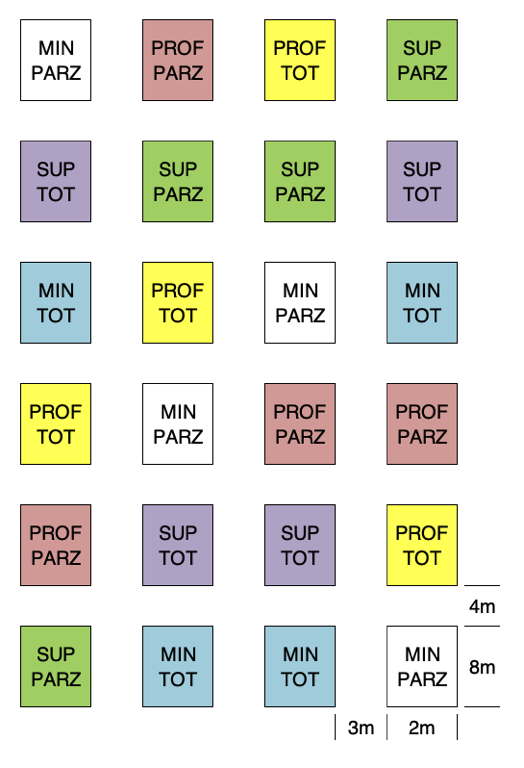
\includegraphics[width=0.90000\textwidth]{_images/Mappa3FATT.png}
\caption{Schema sperimentale fattoriale a blocchi randomizzati per
l'Esempio 3}
\end{figure}

Questo disegno è totalmente appropriato, ma ci costringe a lasciare
parecchio spazio tra una parcella e l'altra, per poter manovrare con la
macchina per la lavorazione del terreno. Sarebbe utile raggruppare le
parcelle caratterizzate dalla stessa lavorazione, in modo da poter
lavorare su superfici più ampie. Ne guadagnerebbe l'uniformità
dell'esperimento e l'accuratezza dei risultati. Possiamo quindi
immaginare un disegno a un fattore, con parcelle di dimensione doppia
(\textbf{main-plots}), sulle quali eseguire, in modo randomizzato le
lavorazioni del terreno. Succesivamente, ogni main-plot può essere
suddivisa in due e, su ognuna delle due metà, possono essere allocati in
modo random i due trattamenti di diserbo. In questo modo ci troviamo ad
operare con parcelle di due dimensioni diverse: le main-plots per le
lavorazioni e le sub-plots per il diserbo. Questo tipo di schema prende
il nome di \textbf{parcella suddivisa} (\textbf{split-plot}), ed è
piuttosto comune nella sperimentazione di pieno campo.

Proviamo ad utilizzare R per redigere il piano sperimentale.

\begin{Shaded}
\begin{Highlighting}[]
\NormalTok{lavorazione <-}\StringTok{ }\KeywordTok{c}\NormalTok{(}\StringTok{"PROF"}\NormalTok{, }\StringTok{"SUP"}\NormalTok{, }\StringTok{"MIN"}\NormalTok{)}
\NormalTok{diserbo <-}\StringTok{ }\KeywordTok{c}\NormalTok{(}\StringTok{"TOT"}\NormalTok{, }\StringTok{"PARZ"}\NormalTok{)}
\NormalTok{designSPLIT <-}\StringTok{ }\KeywordTok{design.split}\NormalTok{(lavorazione, diserbo, }\DataTypeTok{r=}\DecValTok{4}\NormalTok{, }\DataTypeTok{serie=}\DecValTok{2}\NormalTok{, }\DataTypeTok{seed=}\DecValTok{777}\NormalTok{)}
\NormalTok{book <-}\StringTok{ }\NormalTok{designSPLIT}\OperatorTok{$}\NormalTok{book}
\NormalTok{book}
\end{Highlighting}
\end{Shaded}

\begin{verbatim}
##    plots splots block lavorazione diserbo
## 1    101      1     1         SUP    PARZ
## 2    101      2     1         SUP     TOT
## 3    102      1     1        PROF     TOT
## 4    102      2     1        PROF    PARZ
## 5    103      1     1         MIN    PARZ
## 6    103      2     1         MIN     TOT
## 7    104      1     2         SUP    PARZ
## 8    104      2     2         SUP     TOT
## 9    105      1     2         MIN     TOT
## 10   105      2     2         MIN    PARZ
## 11   106      1     2        PROF     TOT
## 12   106      2     2        PROF    PARZ
## 13   107      1     3         MIN     TOT
## 14   107      2     3         MIN    PARZ
## 15   108      1     3         SUP     TOT
## 16   108      2     3         SUP    PARZ
## 17   109      1     3        PROF     TOT
## 18   109      2     3        PROF    PARZ
## 19   110      1     4        PROF    PARZ
## 20   110      2     4        PROF     TOT
## 21   111      1     4         MIN     TOT
## 22   111      2     4         MIN    PARZ
## 23   112      1     4         SUP    PARZ
## 24   112      2     4         SUP     TOT
\end{verbatim}

\begin{figure}
\centering
\includegraphics[width=0.90000\textwidth]{_images/Mappa3SPLIT.png}
\caption{Schema sperimentale split-plot a blocchi randomizzati per
l'Esempio 3}
\end{figure}

In alcune circostanze, soprattutto nelle prove di diserbo chimico,
potrebbe trovare applicazione un altro tipo di schema sperimentale, nel
quale, in ogni blocco, un trattamento viene applicato a tutte le
parcelle di una riga e l'altro trattamento a tutte le parcelle di una
colonna. Ad esempio, il disegno sottostante mostra una prova nella quale
il terreno è stato diserbato in una striscia nel senso della lunghezza
e, dopo il diserbo, le colture sono state seminate in striscia, nel
senso della larghezza. Questo disegno è detto \textbf{strip-plot} ed è
molto comodo perché consente di lavorare velocemente.

\begin{figure}
\centering
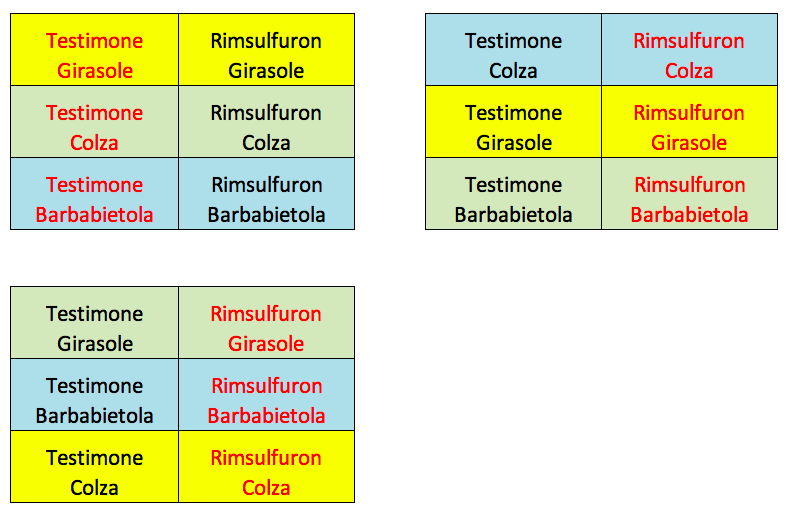
\includegraphics[width=0.90000\textwidth]{_images/MappaStrip.png}
\caption{Schema sperimentale strip-plot}
\end{figure}

\subsubsection{Esempio 4}\label{esempio-4-1}

La prova di erba medica è fondamentalmente un esperimento a blocchi
randomizzati, il cui piano è riportato più sotto. Tuttavia, si tratta di
una coltura poiliennale nella quale ripeteremo le misurazioni ogni anno
sulle stesse parcelle. le misure ripetute non sono randomizzate (non
possono esserlo), ma seguono una metrica temporale. Proprio per questo
sviluppo lungo la scala del tempo, i dati che si raccolgono in questi
esperimenti a misure ripetute sono detti \textbf{dati longitudinali}.
Guardando bene il disegno si capisce anche per si parla di
\textbf{split-plot nel tempo}. Esempi affini sono relativi all'analisi
di accrescimento con misure non distruttive (esempio l'altezza) oppure i
prelievi di terreno a profondità diverse, anche se, in quest'ultimo
caso, la metrica delle misure ripetute è spaziale, non temporale.

Si può notare una certa analogia con il sottocampionamento illsutrato
più sopra, nel senso che vengono prese più misure per parcella.
Tuttavia, bisogna tener presente che nel sottocampionamento le diverse
misure sono solo repliche e non vi è nessuna esigenza di distinguere tra
quelle prese nella stessa parcella. Invece, nel caso delle misure
ripetute ognuna di esse ha interesse individuale, in quanto espressione
di un'anno particolare.

\begin{figure}
\centering
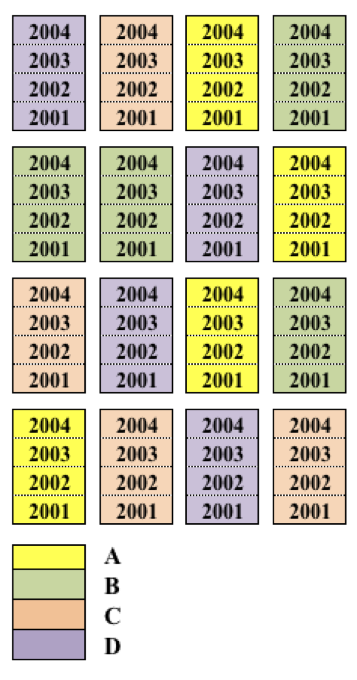
\includegraphics[width=0.90000\textwidth]{_images/Mappa4.png}
\caption{Schema sperimentale a blocchi randomizzati con misure ripetute}
\end{figure}

\subsubsection{Esempio 5}\label{esempio-5-1}

Per questo disegno osservazionale, la mappa non è necessaria. Tuttavia,
si può notare che, in ogni supermercato, abbiamo un disegno a
randomizzazione completa, con tre tipi di confezioni e tre repliche,
cioè nove confezioni scelte a random da un lotto più grande. Insomma, si
tratta di un esperimento ripetuto 9 volte che, pertanto, ha una certa
affinità con l'esperimento ripetuto dell'Esempio 2.

\subsection{Impianto delle prove}\label{impianto-delle-prove}

Da questo punto in poi, subentrano le competenze agronomiche e
fitopatologiche necessarie per codurre gli esperimenti, Mi piace solo
ricordare alcune pratiche usuali nella sperimentazione di pieno campo,
destinate a migliorare l'efficienza della prova.

\begin{enumerate}
\def\labelenumi{\arabic{enumi}.}
\tightlist
\item
  Seminare a densità più alte e poi diradare, per assicurare una
  migliore uniformità di impianto
\item
  Prelevare da ogni parcella più campioni ed, eventualmente,
  omogeneizzarli o mediare i risultati ottenuti (vedi il caso dei 1000
  semi)
\item
  Considerare le caratteristiche naturalmente meno variabili (es. la
  produzione areica e non la produzione per pianta)
\end{enumerate}

Voglio inoltre ricordare che gli esperimenti parcellari configurano una
situazione nella quale, per l'elevata cura che si pone nelle tecniche
agronomiche, si riesce ad ottenere una produttività almeno del 20\%
superiore rispetto a quanto avviene nella normale pratica agricola.

\section{Come scrivere un progetto di ricerca o un report di
ricerca}\label{come-scrivere-un-progetto-di-ricerca-o-un-report-di-ricerca}

Quanto abbiamo finora esposto costituisce uno schema generale che può
essere adottato per redigere un progetto di ricerca o un report sui
risultati ottenuti (tesi, pubblicazione). Bisogna provare che la ricerca
che si è eseguita è precisa, accurata e replicabile/riproducibile e, di
conseguenza, i risultati sono validi.

Nella redazione di un progetto di ricerca o di un report, è fondamentale
tratteggiare bene i seguenti elementi:

\begin{enumerate}
\def\labelenumi{\arabic{enumi}.}
\tightlist
\item
  Titolo della ricerca
\item
  Descrizione del problema e background scientifico
\item
  Ipotesi scientifica, motivazioni e obiettivi
\item
  Tipo di esperimento e durata
\item
  Disegno sperimentale: trattamenti sperimentali (tesi) a confronto con
  dettagli relativi all'applicazione
\item
  Unità sperimentali e criteri per la loro selezione. Dettagli su
  repliche e randomizzazione
\item
  Dettagli su eventuali tecniche di `blocking'
\item
  Variabili da rilevare/rilevate
\item
  Dettagli su come le variabili saranno/sono state rilevate
\item
  Esposizione dei risultati (solo report)
\item
  Discussione (solo report)
\item
  Conclusioni (solo report)
\end{enumerate}

Alcuni aspetti che divengono elemento di valutazione del progetto e/o
del report sono i seguenti:

\begin{enumerate}
\def\labelenumi{\arabic{enumi}.}
\tightlist
\item
  La selezione dei metodi deve essere coerente con gli obiettivi
\item
  Descrizione dettagliata dei materiali e metodi (bisogna che chiunque
  sia in grado di replicare l'esperimento)
\item
  Esposizione dei risultati chiara e convincente
\item
  Discussione approfondita e con molti riferimenti alla letteratura.
\end{enumerate}

\section{Per approfondimenti}\label{per-approfondimenti}

\begin{enumerate}
\def\labelenumi{\arabic{enumi}.}
\tightlist
\item
  Hurlbert, S., 1984. Pseudoreplication and the design of ecological
  experiments. Ecological Monographs, 54, 187-211
\item
  Kuehl, R. O., 2000. Design of experiments: statistical principles of
  research design and analysis. Duxbury Press (CHAPTER 1)
\item
  LeClerg, E.; Leonard, W. \& Clark, A., 1962. Field Plot Technique.
  Burgess Publishing Company, (CHAPTER 3)
\item
  Felipe de Mendiburu (2017). agricolae: Statistical Procedures for
  Agricultural Research. R package, version 1.2-8.
  \url{https://CRAN.R-project.org/package=agricolae}
\end{enumerate}

\chapter{Methods}\label{methods}

We describe our methods in this chapter.

\chapter{Applications}\label{applications}

Some \emph{significant} applications are demonstrated in this chapter.

\section{Example one}\label{example-one}

\section{Example two}\label{example-two}

\chapter{Final Words}\label{final-words}

We have finished a nice book.

\chapter*{References}\label{references}
\addcontentsline{toc}{chapter}{References}


\end{document}
